
%% bare_jrnl.tex
%% V1.4b
%% 2015/08/26
%% by Michael Shell
%% see http://www.michaelshell.org/
%% for current contact information.
%%
%% This is a skeleton file demonstrating the use of IEEEtran.cls
%% (requires IEEEtran.cls version 1.8b or later) with an IEEE
%% journal paper.
%%
%% Support sites:
%% http://www.michaelshell.org/tex/ieeetran/
%% http://www.ctan.org/pkg/ieeetran
%% and
%% http://www.ieee.org/

%%*************************************************************************
%% Legal Notice:
%% This code is offered as-is without any warranty either expressed or
%% implied; without even the implied warranty of MERCHANTABILITY or
%% FITNESS FOR A PARTICULAR PURPOSE! 
%% User assumes all risk.
%% In no event shall the IEEE or any contributor to this code be liable for
%% any damages or losses, including, but not limited to, incidental,
%% consequential, or any other damages, resulting from the use or misuse
%% of any information contained here.
%%
%% All comments are the opinions of their respective authors and are not
%% necessarily endorsed by the IEEE.
%%
%% This work is distributed under the LaTeX Project Public License (LPPL)
%% ( http://www.latex-project.org/ ) version 1.3, and may be freely used,
%% distributed and modified. A copy of the LPPL, version 1.3, is included
%% in the base LaTeX documentation of all distributions of LaTeX released
%% 2003/12/01 or later.
%% Retain all contribution notices and credits.
%% ** Modified files should be clearly indicated as such, including  **
%% ** renaming them and changing author support contact information. **
%%*************************************************************************


% *** Authors should verify (and, if needed, correct) their LaTeX system  ***
% *** with the testflow diagnostic prior to trusting their LaTeX platform ***
% *** with production work. The IEEE's font choices and paper sizes can   ***
% *** trigger bugs that do not appear when using other class files.       ***                          ***
% The testflow support page is at:
% http://www.michaelshell.org/tex/testflow/



\documentclass[journal]{IEEEtran}
%
% If IEEEtran.cls has not been installed into the LaTeX system files,
% manually specify the path to it like:
% \documentclass[journal]{../sty/IEEEtran}


\usepackage[utf8]{inputenc}
\usepackage{graphicx}
\usepackage{subcaption} 
\usepackage{hyperref}
\usepackage{algorithm2e} % For algorithms
\usepackage{amsmath, amssymb, amsthm} % Mathematical packages
\hypersetup{hidelinks=true}    

% Some very useful LaTeX packages include:
% (uncomment the ones you want to load)


% *** MISC UTILITY PACKAGES ***
%
%\usepackage{ifpdf}
% Heiko Oberdiek's ifpdf.sty is very useful if you need conditional
% compilation based on whether the output is pdf or dvi.
% usage:
% \ifpdf
%   % pdf code
% \else
%   % dvi code
% \fi
% The latest version of ifpdf.sty can be obtained from:
% http://www.ctan.org/pkg/ifpdf
% Also, note that IEEEtran.cls V1.7 and later provides a builtin
% \ifCLASSINFOpdf conditional that works the same way.
% When switching from latex to pdflatex and vice-versa, the compiler may
% have to be run twice to clear warning/error messages.






% *** CITATION PACKAGES ***
%
%\usepackage{cite}
% cite.sty was written by Donald Arseneau
% V1.6 and later of IEEEtran pre-defines the format of the cite.sty package
% \cite{} output to follow that of the IEEE. Loading the cite package will
% result in citation numbers being automatically sorted and properly
% "compressed/ranged". e.g., [1], [9], [2], [7], [5], [6] without using
% cite.sty will become [1], [2], [5]--[7], [9] using cite.sty. cite.sty's
% \cite will automatically add leading space, if needed. Use cite.sty's
% noadjust option (cite.sty V3.8 and later) if you want to turn this off
% such as if a citation ever needs to be enclosed in parenthesis.
% cite.sty is already installed on most LaTeX systems. Be sure and use
% version 5.0 (2009-03-20) and later if using hyperref.sty.
% The latest version can be obtained at:
% http://www.ctan.org/pkg/cite
% The documentation is contained in the cite.sty file itself.






% *** GRAPHICS RELATED PACKAGES ***
%
\ifCLASSINFOpdf
  % \usepackage[pdftex]{graphicx}
  % declare the path(s) where your graphic files are
  % \graphicspath{{../pdf/}{../jpeg/}}
  % and their extensions so you won't have to specify these with
  % every instance of \includegraphics
  % \DeclareGraphicsExtensions{.pdf,.jpeg,.png}
\else
  % or other class option (dvipsone, dvipdf, if not using dvips). graphicx
  % will default to the driver specified in the system graphics.cfg if no
  % driver is specified.
  % \usepackage[dvips]{graphicx}
  % declare the path(s) where your graphic files are
  % \graphicspath{{../eps/}}
  % and their extensions so you won't have to specify these with
  % every instance of \includegraphics
  % \DeclareGraphicsExtensions{.eps}
\fi
% graphicx was written by David Carlisle and Sebastian Rahtz. It is
% required if you want graphics, photos, etc. graphicx.sty is already
% installed on most LaTeX systems. The latest version and documentation
% can be obtained at: 
% http://www.ctan.org/pkg/graphicx
% Another good source of documentation is "Using Imported Graphics in
% LaTeX2e" by Keith Reckdahl which can be found at:
% http://www.ctan.org/pkg/epslatex
%
% latex, and pdflatex in dvi mode, support graphics in encapsulated
% postscript (.eps) format. pdflatex in pdf mode supports graphics
% in .pdf, .jpeg, .png and .mps (metapost) formats. Users should ensure
% that all non-photo figures use a vector format (.eps, .pdf, .mps) and
% not a bitmapped formats (.jpeg, .png). The IEEE frowns on bitmapped formats
% which can result in "jaggedy"/blurry rendering of lines and letters as
% well as large increases in file sizes.
%
% You can find documentation about the pdfTeX application at:
% http://www.tug.org/applications/pdftex





% *** MATH PACKAGES ***
%
%\usepackage{amsmath}
% A popular package from the American Mathematical Society that provides
% many useful and powerful commands for dealing with mathematics.
%
% Note that the amsmath package sets \interdisplaylinepenalty to 10000
% thus preventing page breaks from occurring within multiline equations. Use:
%\interdisplaylinepenalty=2500
% after loading amsmath to restore such page breaks as IEEEtran.cls normally
% does. amsmath.sty is already installed on most LaTeX systems. The latest
% version and documentation can be obtained at:
% http://www.ctan.org/pkg/amsmath





% *** SPECIALIZED LIST PACKAGES ***
%
%\usepackage{algorithmic}
% algorithmic.sty was written by Peter Williams and Rogerio Brito.
% This package provides an algorithmic environment fo describing algorithms.
% You can use the algorithmic environment in-text or within a figure
% environment to provide for a floating algorithm. Do NOT use the algorithm
% floating environment provided by algorithm.sty (by the same authors) or
% algorithm2e.sty (by Christophe Fiorio) as the IEEE does not use dedicated
% algorithm float types and packages that provide these will not provide
% correct IEEE style captions. The latest version and documentation of
% algorithmic.sty can be obtained at:
% http://www.ctan.org/pkg/algorithms
% Also of interest may be the (relatively newer and more customizable)
% algorithmicx.sty package by Szasz Janos:
% http://www.ctan.org/pkg/algorithmicx




% *** ALIGNMENT PACKAGES ***
%
%\usepackage{array}
% Frank Mittelbach's and David Carlisle's array.sty patches and improves
% the standard LaTeX2e array and tabular environments to provide better
% appearance and additional user controls. As the default LaTeX2e table
% generation code is lacking to the point of almost being broken with
% respect to the quality of the end results, all users are strongly
% advised to use an enhanced (at the very least that provided by array.sty)
% set of table tools. array.sty is already installed on most systems. The
% latest version and documentation can be obtained at:
% http://www.ctan.org/pkg/array


% IEEEtran contains the IEEEeqnarray family of commands that can be used to
% generate multiline equations as well as matrices, tables, etc., of high
% quality.




% *** SUBFIGURE PACKAGES ***
%\ifCLASSOPTIONcompsoc
%  \usepackage[caption=false,font=normalsize,labelfont=sf,textfont=sf]{subfig}
%\else
%  \usepackage[caption=false,font=footnotesize]{subfig}
%\fi
% subfig.sty, written by Steven Douglas Cochran, is the modern replacement
% for subfigure.sty, the latter of which is no longer maintained and is
% incompatible with some LaTeX packages including fixltx2e. However,
% subfig.sty requires and automatically loads Axel Sommerfeldt's caption.sty
% which will override IEEEtran.cls' handling of captions and this will result
% in non-IEEE style figure/table captions. To prevent this problem, be sure
% and invoke subfig.sty's "caption=false" package option (available since
% subfig.sty version 1.3, 2005/06/28) as this is will preserve IEEEtran.cls
% handling of captions.
% Note that the Computer Society format requires a larger sans serif font
% than the serif footnote size font used in traditional IEEE formatting
% and thus the need to invoke different subfig.sty package options depending
% on whether compsoc mode has been enabled.
%
% The latest version and documentation of subfig.sty can be obtained at:
% http://www.ctan.org/pkg/subfig




% *** FLOAT PACKAGES ***
%
%\usepackage{fixltx2e}
% fixltx2e, the successor to the earlier fix2col.sty, was written by
% Frank Mittelbach and David Carlisle. This package corrects a few problems
% in the LaTeX2e kernel, the most notable of which is that in current
% LaTeX2e releases, the ordering of single and double column floats is not
% guaranteed to be preserved. Thus, an unpatched LaTeX2e can allow a
% single column figure to be placed prior to an earlier double column
% figure.
% Be aware that LaTeX2e kernels dated 2015 and later have fixltx2e.sty's
% corrections already built into the system in which case a warning will
% be issued if an attempt is made to load fixltx2e.sty as it is no longer
% needed.
% The latest version and documentation can be found at:
% http://www.ctan.org/pkg/fixltx2e


%\usepackage{stfloats}
% stfloats.sty was written by Sigitas Tolusis. This package gives LaTeX2e
% the ability to do double column floats at the bottom of the page as well
% as the top. (e.g., "\begin{figure*}[!b]" is not normally possible in
% LaTeX2e). It also provides a command:
%\fnbelowfloat
% to enable the placement of footnotes below bottom floats (the standard
% LaTeX2e kernel puts them above bottom floats). This is an invasive package
% which rewrites many portions of the LaTeX2e float routines. It may not work
% with other packages that modify the LaTeX2e float routines. The latest
% version and documentation can be obtained at:
% http://www.ctan.org/pkg/stfloats
% Do not use the stfloats baselinefloat ability as the IEEE does not allow
% \baselineskip to stretch. Authors submitting work to the IEEE should note
% that the IEEE rarely uses double column equations and that authors should try
% to avoid such use. Do not be tempted to use the cuted.sty or midfloat.sty
% packages (also by Sigitas Tolusis) as the IEEE does not format its papers in
% such ways.
% Do not attempt to use stfloats with fixltx2e as they are incompatible.
% Instead, use Morten Hogholm'a dblfloatfix which combines the features
% of both fixltx2e and stfloats:
%
% \usepackage{dblfloatfix}
% The latest version can be found at:
% http://www.ctan.org/pkg/dblfloatfix




%\ifCLASSOPTIONcaptionsoff
%  \usepackage[nomarkers]{endfloat}
% \let\MYoriglatexcaption\caption
% \renewcommand{\caption}[2][\relax]{\MYoriglatexcaption[#2]{#2}}
%\fi
% endfloat.sty was written by James Darrell McCauley, Jeff Goldberg and 
% Axel Sommerfeldt. This package may be useful when used in conjunction with 
% IEEEtran.cls'  captionsoff option. Some IEEE journals/societies require that
% submissions have lists of figures/tables at the end of the paper and that
% figures/tables without any captions are placed on a page by themselves at
% the end of the document. If needed, the draftcls IEEEtran class option or
% \CLASSINPUTbaselinestretch interface can be used to increase the line
% spacing as well. Be sure and use the nomarkers option of endfloat to
% prevent endfloat from "marking" where the figures would have been placed
% in the text. The two hack lines of code above are a slight modification of
% that suggested by in the endfloat docs (section 8.4.1) to ensure that
% the full captions always appear in the list of figures/tables - even if
% the user used the short optional argument of \caption[]{}.
% IEEE papers do not typically make use of \caption[]'s optional argument,
% so this should not be an issue. A similar trick can be used to disable
% captions of packages such as subfig.sty that lack options to turn off
% the subcaptions:
% For subfig.sty:
% \let\MYorigsubfloat\subfloat
% \renewcommand{\subfloat}[2][\relax]{\MYorigsubfloat[]{#2}}
% However, the above trick will not work if both optional arguments of
% the \subfloat command are used. Furthermore, there needs to be a
% description of each subfigure *somewhere* and endfloat does not add
% subfigure captions to its list of figures. Thus, the best approach is to
% avoid the use of subfigure captions (many IEEE journals avoid them anyway)
% and instead reference/explain all the subfigures within the main caption.
% The latest version of endfloat.sty and its documentation can obtained at:
% http://www.ctan.org/pkg/endfloat
%
% The IEEEtran \ifCLASSOPTIONcaptionsoff conditional can also be used
% later in the document, say, to conditionally put the References on a 
% page by themselves.




% *** PDF, URL AND HYPERLINK PACKAGES ***
%
%\usepackage{url}
% url.sty was written by Donald Arseneau. It provides better support for
% handling and breaking URLs. url.sty is already installed on most LaTeX
% systems. The latest version and documentation can be obtained at:
% http://www.ctan.org/pkg/url
% Basically, \url{my_url_here}.




% *** Do not adjust lengths that control margins, column widths, etc. ***
% *** Do not use packages that alter fonts (such as pslatex).         ***
% There should be no need to do such things with IEEEtran.cls V1.6 and later.
% (Unless specifically asked to do so by the journal or conference you plan
% to submit to, of course. )


% correct bad hyphenation here
\hyphenation{op-tical net-works semi-conduc-tor}


\begin{document}
%
% paper title
% Titles are generally capitalized except for words such as a, an, and, as,
% at, but, by, for, in, nor, of, on, or, the, to and up, which are usually
% not capitalized unless they are the first or last word of the title.
% Linebreaks \\ can be used within to get better formatting as desired.
% Do not put math or special symbols in the title.
\title{Training a Gaming Agent on Brainwaves}
%
%
% author names and IEEE memberships
% note positions of commas and nonbreaking spaces ( ~ ) LaTeX will not break
% a structure at a ~ so this keeps an author's name from being broken across
% two lines.
% use \thanks{} to gain access to the first footnote area
% a separate \thanks must be used for each paragraph as LaTeX2e's \thanks
% was not built to handle multiple paragraphs
%

\author{Bartolomé Francisco, Moreno Juan,  Navas Natalia, Vitali José, \\
Ramele~Rodrigo,~\IEEEmembership{Member,~IEEE,} 
        Santos~Juan~Miguel% <-this % stops a space
\thanks{R. Ramele and J.M.Santos are with the Department
of Computer Engineering, Instituto Tecnológico de Buenos Aires(ITBA), Argentina,
e-mail: rramele@itba.edu.ar.}% <-this % stops a space
\thanks{Manuscript received April 19, 2005; revised August 26, 2015.}}

% note the % following the last \IEEEmembership and also \thanks - 
% these prevent an unwanted space from occurring between the last author name
% and the end of the author line. i.e., if you had this:
% 
% \author{....lastname \thanks{...} \thanks{...} }
%                     ^------------^------------^----Do not want these spaces!
%
% a space would be appended to the last name and could cause every name on that
% line to be shifted left slightly. This is one of those "LaTeX things". For
% instance, "\textbf{A} \textbf{B}" will typeset as "A B" not "AB". To get
% "AB" then you have to do: "\textbf{A}\textbf{B}"
% \thanks is no different in this regard, so shield the last } of each \thanks
% that ends a line with a % and do not let a space in before the next \thanks.
% Spaces after \IEEEmembership other than the last one are OK (and needed) as
% you are supposed to have spaces between the names. For what it is worth,
% this is a minor point as most people would not even notice if the said evil
% space somehow managed to creep in.



% The paper headers
\markboth{IEEE Transactions on Games}%
{Shell \MakeLowercase{\textit{et al.}}: Bare Demo of IEEEtran.cls for IEEE Journals}
% The only time the second header will appear is for the odd numbered pages
% after the title page when using the twoside option.
% 
% *** Note that you probably will NOT want to include the author's ***
% *** name in the headers of peer review papers.                   ***
% You can use \ifCLASSOPTIONpeerreview for conditional compilation here if
% you desire.




% If you want to put a publisher's ID mark on the page you can do it like
% this:
%\IEEEpubid{0000--0000/00\$00.00~\copyright~2015 IEEE}
% Remember, if you use this you must call \IEEEpubidadjcol in the second
% column for its text to clear the IEEEpubid mark.



% use for special paper notices
%\IEEEspecialpapernotice{(Invited Paper)}




% make the title area
\maketitle

% As a general rule, do not put math, special symbols or citations
% in the abstract or keywords.
\begin{abstract}
The field of Brain Computer Interfaces (BCI) has seen a bloom in the past few years. One of its applications is the training of systems using signals originated from the human brain. Out of all the methods used to acquire information from the central nervous system, the one that has gained most popularity is Electroencephalography (EEG), mainly because of its effectiveness, low cost and its noninvasive characteristic.
Event-related potential (ERP) are brain signals found on EEG that are time-locked to a particular event. Error-related potential (ErrP) are a particular type of ERP that  can be elicited by a person who attends a recognizable error. When subjects observe an agent who makes a mistake this potential can be discerned by analyzing the signals which are directly related with the cognitive interpretation of an erroneous outcome or decision.
Reinforcement Learning (RL) is an Artificial Intelligence approach where an agent tries to maximize rewards obtained while interacting with an unknown environment.  In this work, a gaming agent is trained using RL, and the feedback obtained from brainwaves of human critic observers.  Results show that there is an effective transfer of information and that the agent learns successfully to solve the game efficiently.
\end{abstract}

% Note that keywords are not normally used for peerreview papers.
\begin{IEEEkeywords}
ErrP, BCI, EEG, RL, Agent, AI
\end{IEEEkeywords}



% For peer review papers, you can put extra information on the cover
% page as needed:
% \ifCLASSOPTIONpeerreview
% \begin{center} \bfseries EDICS Category: 3-BBND \end{center}
% \fi
%
% For peerreview papers, this IEEEtran command inserts a page break and
% creates the second title. It will be ignored for other modes.
\IEEEpeerreviewmaketitle



\section{Introduction}


% You must have at least 2 lines in the paragraph with the drop letter
% (should never be an issue)
\IEEEPARstart{T}{he} effectiveness of today's human–machine interaction and artificial intelligence is limited by a communication bottleneck as humans are required to translate high-level concepts into a machine-mandated sequence of instructions~\cite{Xu2020,CURSOR-CONTROL-PAPER}.   This work tackles this problem by exploring the use of brain signals as an interface between humans and computers, trying to provide information to the system without explicit communication from the user.   

On the other hand, video games has been used widely as tools to test new means of interactions\cite{REF}. Gaming agents are computer programs that can sense the game environment, process information, and interact with a computer game, behaving like a real user playing the game.

In this work, the feedback obtained from an observational human critic (OHC) in the form of electroencephalographic (EEG) signals is used to evaluate the operational performance of a gaming agent.  Observational human critics are silent subjects observing a computer gaming agent playing the game. In this set up, gaming agents can be trained using only signals components called Error-related Potentials (ErrP) that can be identified from their brain signals.   This type of signals can be found on EEG traces and are elicited when a subject is aware of the presence of an unexpected outcome, which she/he identifies as an error.  It is currently an extensive area of research in the neuroscience community~\cite{Holroyd2009}.  

Error-related Potentials can be detected by signal processing and machine learning techniques~\cite{EERP-PAPER} and they are also used in Brain-Computer Interfaces (BCI) to implement or enhance artificial communication channels~\cite{Chavarriaga2014}.

In order to train the agent, Reinforcement Learning (RL)~\cite{Santos1999,Sutton2018} comes as a natural solution for this scenario from the field of Artificial Intelligence.  This is an algorithmic learning strategy that can be established by mimicking how biological agents learn from its environment by exploring it and getting feedback rewards, either negative or positive.  This strategy aims to maximize the amount of positive rewards while keeping the number of negative feedback low.  Thus, the learning problem is  posed as a mere stochastic optimization strategy~\cite{sutton2018reinforcement}.  Recently, this technique has been used extensively in the context of recent advances in artificial intelligence~\cite{REF}. Nonneglected is the influence of DeepBrain's AlphaGo project, which was the first to reach a very high proficiency when it won the complex game Go against several world champions~\cite{ALPHA-GO}.

%By using variants of this technique, in 2015 AlphaGo won 5 matches against 3-times European Champion, Mr Fan Hui. AlphaGo then went on to compete against Mr Lee Sedol, winner of 18 world titles and considered to be the greatest player until then, and won 4 out of 5 matches in 2016 \cite{ALPHA-GO}.

Expandir todos los trabajos que se hacen en BCI que es cierto que son muchísimo.s

To assess air traffic controllers decissions~\cite{Goh2019}.  to categorise actions as errors

In the context of Brain Computer Interfaces a growing number of studies have demonstrated the feasibility of using ErrPs as detection for RL tasks.\cite{Wirth2020}.  To enhance robotic behaviour\cite{Luo2019}.

Previous research has explored the usage of RL with reward signals based on brain activity, recorded by an EEG-based BCI system during task execution. The papers \cite{ROBOT-CONTROL-PAPER,Kim2017,Omedes2013} have successfully demonstrated that a robot can be controlled by obtaining a reward signal from a person's brain activity which is observing the robot solve a task.  Other approaches have used the signal as an important feedback for human-robot interaction or to implement shared-control strategies~\cite{Schiatti2018}.  Additionally, ErrPs have also been used in the context of games as an additional feedback channel that can be explored to enhance gaming experience~\cite{Plass-OudeBos2010,kober2018bci}.  In this same line, the objective of this work is to use the information extracted from brainwaves to enhance the performance of a gaming agent, replicating and extending the usage of this signal.

Therefore, the two contributions of this work are (1) bla bla bla bla bla bla bla bla, (2) 


% An example of a floating figure using the graphicx package.
% Note that \label must occur AFTER (or within) \caption.
% For figures, \caption should occur after the \includegraphics.
% Note that IEEEtran v1.7 and later has special internal code that
% is designed to preserve the operation of \label within \caption
% even when the captionsoff option is in effect. However, because
% of issues like this, it may be the safest practice to put all your
% \label just after \caption rather than within \caption{}.
%
% Reminder: the "draftcls" or "draftclsnofoot", not "draft", class
% option should be used if it is desired that the figures are to be
% displayed while in draft mode.
%
%\begin{figure}[!t]
%\centering
%\includegraphics[width=2.5in]{myfigure}
% where an .eps filename suffix will be assumed under latex, 
% and a .pdf suffix will be assumed for pdflatex; or what has been declared
% via \DeclareGraphicsExtensions.
%\caption{Simulation results for the network.}
%\label{fig_sim}
%\end{figure}

% Note that the IEEE typically puts floats only at the top, even when this
% results in a large percentage of a column being occupied by floats.


% An example of a double column floating figure using two subfigures.
% (The subfig.sty package must be loaded for this to work.)
% The subfigure \label commands are set within each subfloat command,
% and the \label for the overall figure must come after \caption.
% \hfil is used as a separator to get equal spacing.
% Watch out that the combined width of all the subfigures on a 
% line do not exceed the text width or a line break will occur.
%
%\begin{figure*}[!t]
%\centering
%\subfloat[Case I]{\includegraphics[width=2.5in]{box}%
%\label{fig_first_case}}
%\hfil
%\subfloat[Case II]{\includegraphics[width=2.5in]{box}%
%\label{fig_second_case}}
%\caption{Simulation results for the network.}
%\label{fig_sim}
%\end{figure*}
%
% Note that often IEEE papers with subfigures do not employ subfigure
% captions (using the optional argument to \subfloat[]), but instead will
% reference/describe all of them (a), (b), etc., within the main caption.
% Be aware that for subfig.sty to generate the (a), (b), etc., subfigure
% labels, the optional argument to \subfloat must be present. If a
% subcaption is not desired, just leave its contents blank,
% e.g., \subfloat[].


% An example of a floating table. Note that, for IEEE style tables, the
% \caption command should come BEFORE the table and, given that table
% captions serve much like titles, are usually capitalized except for words
% such as a, an, and, as, at, but, by, for, in, nor, of, on, or, the, to
% and up, which are usually not capitalized unless they are the first or
% last word of the caption. Table text will default to \footnotesize as
% the IEEE normally uses this smaller font for tables.
% The \label must come after \caption as always.
%
%\begin{table}[!t]
%% increase table row spacing, adjust to taste
%\renewcommand{\arraystretch}{1.3}
% if using array.sty, it might be a good idea to tweak the value of
% \extrarowheight as needed to properly center the text within the cells
%\caption{An Example of a Table}
%\label{table_example}
%\centering
%% Some packages, such as MDW tools, offer better commands for making tables
%% than the plain LaTeX2e tabular which is used here.
%\begin{tabular}{|c||c|}
%\hline
%One & Two\\
%\hline
%Three & Four\\
%\hline
%\end{tabular}
%\end{table}


% Note that the IEEE does not put floats in the very first column
% - or typically anywhere on the first page for that matter. Also,
% in-text middle ("here") positioning is typically not used, but it
% is allowed and encouraged for Computer Society conferences (but
% not Computer Society journals). Most IEEE journals/conferences use
% top floats exclusively. 
% Note that, LaTeX2e, unlike IEEE journals/conferences, places
% footnotes above bottom floats. This can be corrected via the
% \fnbelowfloat command of the stfloats package.

In Section \ref{section:materials} the general layout of the cognitive game is described. Section \ref{section:calibration} outlines the processing pipeline used to detect ErrP components. The following Section \ref{learning} describes the agent learning phase.   Results and Conclusions are exposed in Sections \ref{results} and \ref{conclusions}.

\section{Materials and Methods}
\label{section:materials}

This first part consists in collecting signals from a person's brainwaves while they are watching a game where the agent knows the game rules but not how to win it. Hence, the agent can learn the winning strategy using the person's feedback to improve its own performance. This section describes the process of obtaining the person's brain signals that are used to make the agent more efficient.

\begin{figure*}
    \centering
    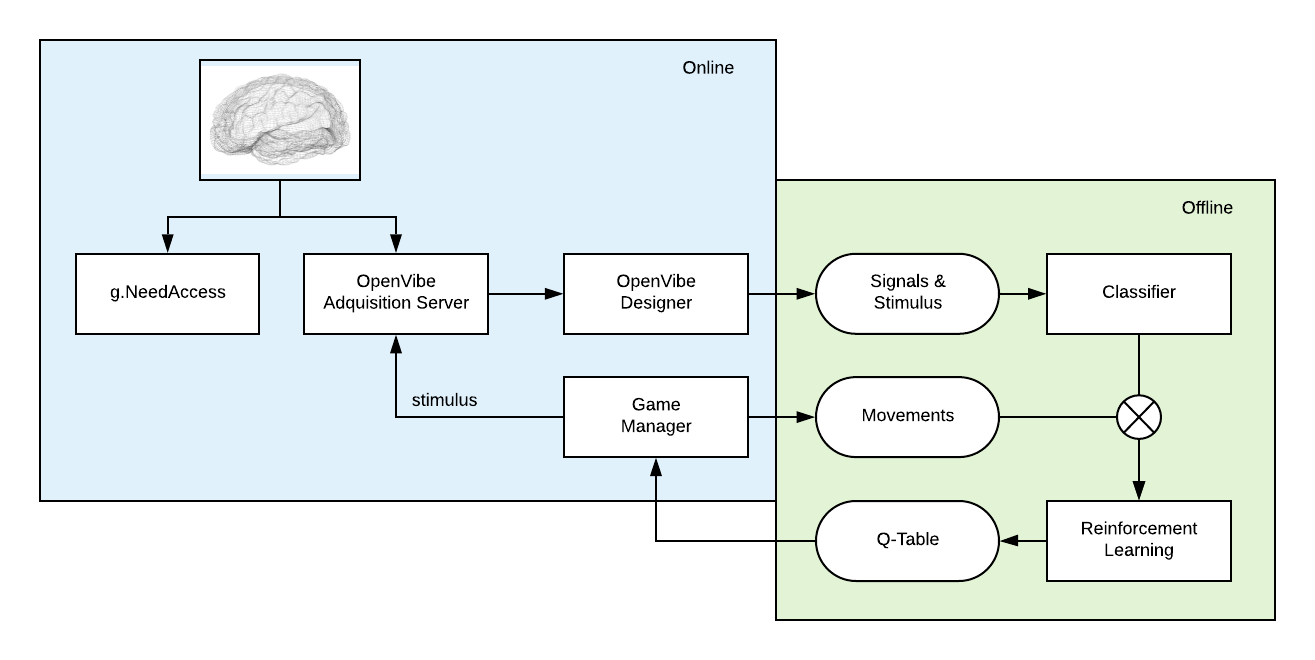
\includegraphics[width=\textwidth]{Images/complete_flow.png}
    \caption{Overview of the experimental procedure. Brainwaves are obtained by the OpenVibe Acquisition Server.  The Game Manager is responsible for generating the game screen, the game mechanics, and the game movements performed by the gaming agent.  It is also connected to the Acquisition Server to send stimulus information.  The captured information is stored by the OpenVibe Designer.  Offline, EEG signals are classified and they are linked to each game movement calculated by the Game Manager to determine proper rewards for each action.  This information is used by a Reinforcement Learning algorithm to learn a Q-Table to improve the performance of the agent that plays the game.}
    \label{diag:complete_flow}
\end{figure*}

The experimental procedure is summarized in Figure \ref{diag:complete_flow}. The central part is the retrieval of the observation human critic's brain activity.  This process is called brainwave session. Subjects are recruited voluntarily. They are given a consent form with questions regarding their health (previous health issues and particular visual sensitivity), habits (sleeping hours, caffeine and alcohol consumption), as well as an approval petition to collect the required data. The brainwave sessions are performed with 8 subjects, 5 males and 3 females, average age 25.12 years, standard deviation 1.54 years, range of 22-28 years. All subjects have normal vision, are right-handed and have no history of neurological disorders.

After the form is filled out, a short description of the procedure is given to each subject. They are only told that the objective of the agent is to reach the goal and the four movements that the agent can make. When this concludes, the subject is introduced to the wireless digital EEG device (g.Nautilus, g.Tec, Austria) that she/he has to wear during the brainwave session. It has eight electrodes (g.LADYbird, g.Tec, Austria) on the positions Fz, Cz, Pz, Oz, P3, P4, PO7 and PO8, identified according to the 10-20 International System, with a reference set to the right ear lobe and ground set as the AFz position. The electrode contact points are adjusted applying conductive gel until the impedance values displayed by the program g.NeedAccess (g.Tec, Austria) are within the desired range. This process takes between 10 to 15 minutes. After this step, the subject is instructed to close their eyes and the same program is used to check the live channel values so that there are no dead ones and the expected values are displayed for eye movements or muscle chewing.

Once the headset is correctly applied, the OpenVibe Acquisition Server program, from the OpenVibe platform~\cite{OPEN-VIBE-PAPER}, is launched and configured with a sampling rate of $250$~Hz. A $50$~Hz notch filter is applied to filter out power line noise. An additional bandpass filter between $0.5$~Hz and $60$~Hz is applied as well. Data is handled and processed with the OpenVibe Designer, from the same platform, using 8 channels for the brain data (one channel per electrode) and an additional channel for the stimulus, which corresponds to a game movement performed by the agent.  After everything is connected, the subject seats in a comfortable chair in front of a computer screen. The brightness of the screen is set to the maximum setting to avoid any visual inconvenience in which the subject can not distinguish the components of the game that appear on the screen.  This dataset has been published on the IEEE DataPort initiative~\cite{6emh-wb46-19}.


The Acquisition Server has the responsibility of receiving and synchronizing the signal data from the headset and any event information from the game, and transfers it to the OpenVibe Designer application. When the subject is ready, the Game Manager and the OpenVibe Designer programs are launched and configured to communicate with the previously mentioned Acquisition Server. A brainwave session consists of several experiences, each one being a game run.  At the end, all the sequence of game movements and the signal data of each run are saved for offline processing.

%ACA For each run, the signals and stimulus information are then passed to the classification module that uses them to train the classifier.  After this step is finished, the game movements and the trained classifier are used to update a Q-Table for each experience. Lastly, the calculated Q-Table is used to test if the agent has boosted its performance while playing the game. This module is explained in Section \ref{q_learning_step}.

\subsection{Cognitive Game Procedure}
\label{cognitive_experiment_details}
%This section details the game system characteristics, the brainwave session process and the retrieval and analysis of the generated data from the subjects interaction with the system.

\label{cognitive_experiment_system}{
The game parsimoniously consists of a $5x5$ grid of grey circular spots with a black background.  A blue spot indicates current position of the agent whereas a green spot represents the goal, as shown in Figure  \ref{fig:game_representation}. The agent's objective is to reach the goal. The circular spot representing the goal remains static at the bottom-right position of the grid, while the one representing the position of the agent always starts at the upper-left position of the grid.  When the agent reaches the goal, the position where the agent and the goal are located turns red, showing that the experience has ended. There are four possible movements that the agent can perform: it can go upwards, downwards, towards the left and towards the right, and those movements are bounded to avoid the agent from leaving the grid. The movement direction is selected randomly and is executed once every 2 seconds.  At the end, there is a pause of 5 seconds before the next experience starts. Each time an agent moves, the Game Manager program sends an event marker to the Acquisition Server.  This is considered as a stimulus to the observational human critic.  The experience is designed for it to be evident whenever there is an error (i.e. the agent moves away from the objective) so the subject can notice it immediately after the stimulus is presented, possibly triggering the expected cognitive response, which can be imprinted as an ErrP component within the EEG stream.

\begin{figure}[h!]
\begin{subfigure}{0.5\textwidth}
\centering 
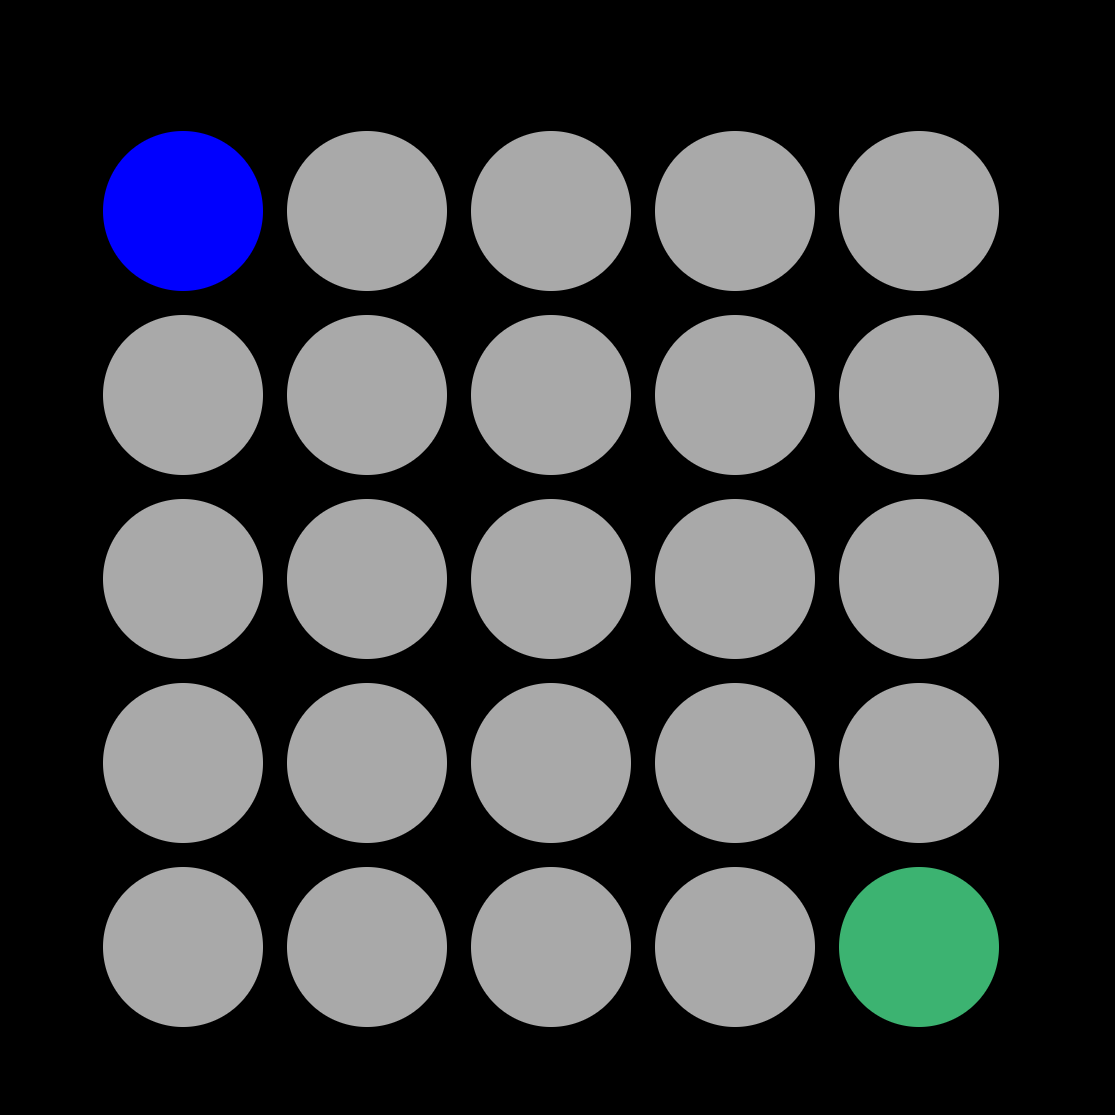
\includegraphics[scale=0.2]{Images/grid_initial_state.png}
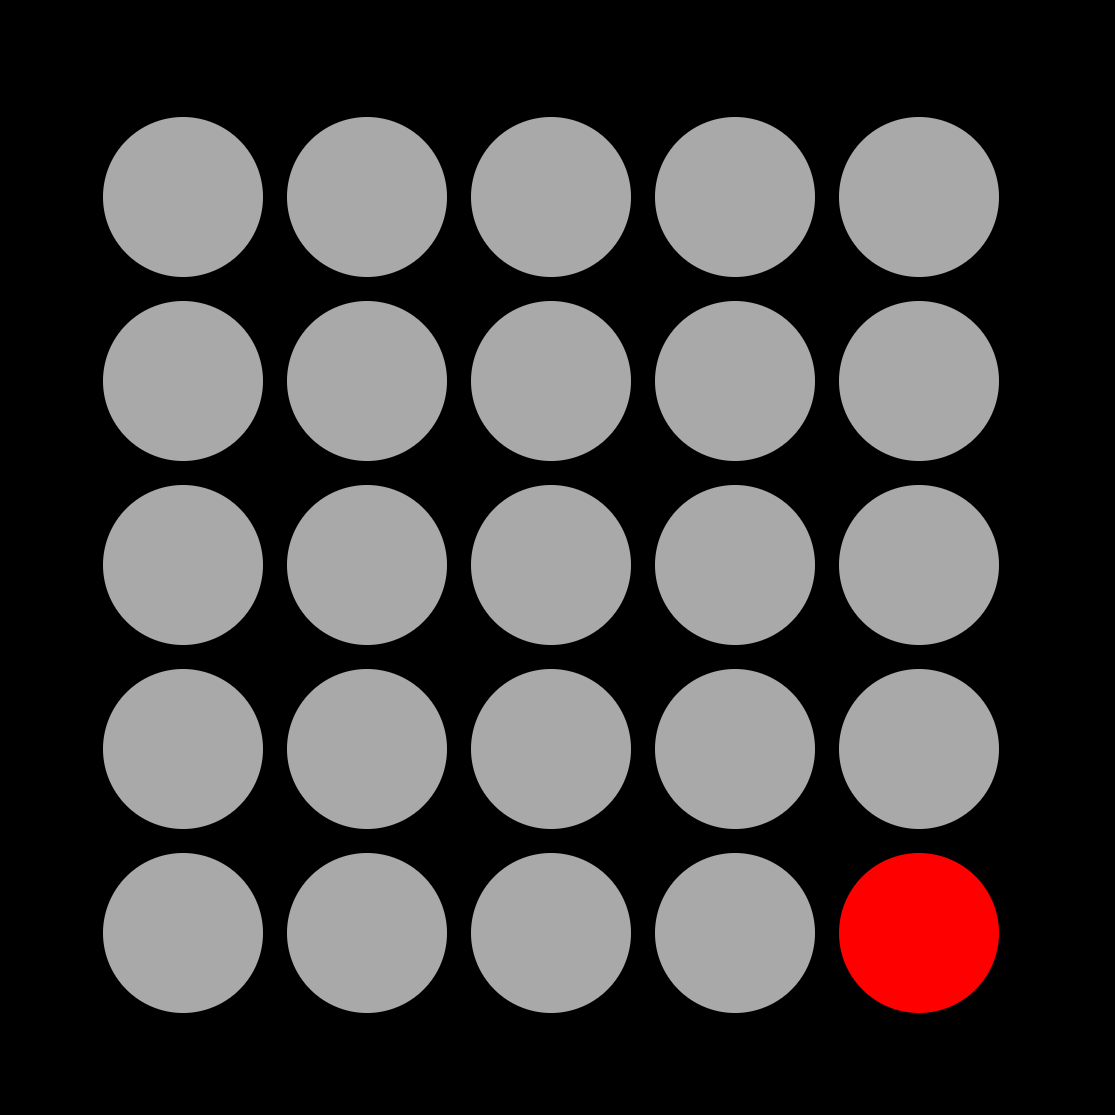
\includegraphics[scale=0.2]{Images/grid_end_state.png}
\end{subfigure}
\centering 
\caption{Grid system representation used in the Cognitive Game Experience. The blue spot represents the initial location while the green spot represents the target location. Once the agent reaches the target spot, its color turns red to indicate the end of the play.}
\label{fig:game_representation}
\end{figure}

%\section{Calibration}
%\label{section:calibration}

%The first step in order to be able to find ErrP signals is to choose the most efficient algorithm, and the proper calibration. In order to do this different parameters are tested for a set of algorithms and for each individual subject. Initially a sub-selection of experiments is used to define a subset of parameters to test with, and then all the data is tested with this subset of parameters.

\section{Signal Processing, Segmentation and Classification}
\label{section:calibration}

To aid in detecting the ErrP response, an offline processing pipeline and classifier is constructed to identify whether the action taken by the agent is an error or not, from the human observer point of view. It is developed in Python using the "MNE" software platform \cite{MNE-PYTHON}, which is a package designed specifically for processing EEG and Magnetoencephalography data, and built upon the machine learning library Scikit-Learn~\cite{scikit-learn}.

This pipeline consists of the offline processing of the collected signals in order to train a classifier that can decide whether an error potential is triggered. Firstly, the output of a brainwave session is read and an additional band pass filter of 0.1-20.0Hz is applied to the signal. Samples that correspond to the start of an event are tagged using the data from the stimulus channel.

After the data is loaded and tagged, epochs are extracted from the raw data. Epochs consist of all the sample points that take place between the start of the event and 2 seconds later (time for each action to take place), resulting in 500 samples per channel, as the sample frequency is 250 Hz. Thus, each epoch is composed of a matrix $500$ x $8$ channels.

Samples that do not correspond to an epoch (located beyond the 2 seconds frame after the onset of the event) are not used. Also, epochs referring to the start or finish of the experience are excluded. This is done because the start and the end of the experience doesn't involve the agent taking an action.

In this way, the raw data of a brainwave session is processed into an array of experiences where each element is an array of epochs tagged with a number specifying the prediction of the classifier, i.e. if the epoch corresponds to an action that made the agent moves further from the goal (hit) or an action that made the agent moves closer to the goal (no-hit). The ErrP is expected to be found in hits. To get the data ready for classification, the stimulus channel is removed in order to classify the signals using only the EEG data. Each epoch is regularized using a MinMaxScaler, i.e. substracting the minimun value in the epoch and dividing by the signal peak-to-peak amplitude~\cite{Zhou2019}.  The eight channels are concatenated using the  MNE Vectorizer function to transform the data matrix into a single array sample. Lastly, this data is used by the classification module as information to train and test a classifier. Four different classification algorithms are used.  Logistic Regression, Multi-layer Perceptron with a hidden layer of 100 neurons (i.e. default values for the Scikit-Learn MLPClassifier), Random Forest and finally a linear kernel Support Vector Classifier (i.e. SVM)~\cite{Lotte2018}.  

%Vectorized epochs are used in the final classification step.  

%and finally the logistic regression classifier.  Even tough the classification accuracy is low, the information is enough to have valid rewards that can be used to retrieve the information.

%a classifier is trained for each subject and then epochs from their experiences are classified. These classifications are then used by a reinforcement learning algorithm to train the agent. This last algorithm is explained in detail in section \ref{q_learning_step}.

\section{Reinforcement Learning}
\label{learning}

Each experience consists of a list of game movement configurations and the associated epochs obtained from subject's brainwaves.  The set of experiences of each subject is split into training and testing.  Training experiences are used to train the classifier, whereas test experiences are used to test its performance.  After a classifier is trained, the epochs of the experience are classified as hit or no-hit.  A reward for each movement in the game run is produced, based on the classification of the epoch that correspond to that movement.  The reward can either be -1 when the event is classified as a hit or 0 when it is classified as a no-hit. The accuracy of this rewards depends on the performance of the classifier. The list of game movements and their associated reward information are used to train the agent by a variant of Reinforcement Learning called Q-Learning algorithm.

%The set of experiences of each subject is split into training and testing, so that the results of the classification can then be used to improve the performance of the agent. Each experience includes an ordered list of extracted epochs for each movement that the agent carried out plus the game state information, i.e. the movement specification.  

%After a classifier is trained, the epochs of the experience are classified as hit or no-hit.  With the game state information and the classification of the test data of an experience, a reward file is composed. This file specifies a reward for each movement in the game run, based on the classification of the event that corresponds to that movement. The reward can either be -1 when the event is classified as a hit or 0 when it is classified as a no-hit. The accuracy of this rewards depends on the performance of the classifier. This reward file is used by the a variant of a Reinforcement Learning algorithm called Q-Learning algorithm.


\subsection{Q-Learning}{
\label{q_learning_step}

Q-Learning~\cite{Watkins1992} is a form of model-free reinforcement learning algorithm where an agent tries an action at a particular state and evaluate its consequences in terms of the reward or penalty it receives.  In order to represent rewards, a matrix $Q(s,a)$ is used, where rows correspond to all the possible states, whereas columns represent all possible actions.  This matrix is known as a Q-Table.  The algorithm proceeds by randomly choosing what action to do and updating iteratively the Q-Table based on the received reward $r$ by the following equation

\begin{equation}
    Q(s,a) \leftarrow Q(s,a) + \alpha[r+\gamma* \max_{\tilde{a}} Q(\tilde{s}, \tilde{a})-Q(s, a) ]
    \label{equ:update_q_table}
\end{equation}

\noindent where $s$ is the current state, $a$ is the action, $\alpha$ represents the learning rate and $\gamma$ represents the discount factor, a value between 0 and 1 that determines the importance of long term results versus immediate rewards.  Hence,  $Q(s,a)$  is the expected value of the sum of discounted rewards that the agent will receive if in the $s$ state, it takes the action $a$ according to this policy.  Once the environment has been extensively explored and the Q-Table has been obtained, the action chosen for a given state is the one that maximizes the expected reward according to the Q-Table matrix.

The algorithm is developed in Python and uses the OpenAI Gym toolkit~\cite{openai}. Gym is a toolkit for developing and comparing reinforcement learning algorithms. It makes no assumptions about the structure of an agent, and is compatible with any numerical computation library, such as TensorFlow or Theano~\cite{tensorflow2015-whitepaper}.

\subsection{Agent Learning}
\label{q_learning_step_alg}
The Q-Table is initialized with zeros, unless a preexisting Q-Table is passed as a parameter.  For the agent, in order to learn from the feedback generated by the subject, the Q-Table is not used to determine the action to take at a given state. Instead, the policy which determines which action to take in a particular state is given by the agent's actions taken from the brainwave session results. This allows to learn the Q-Table based on the subject's feedback from the movements the agent took, which are chosen pseudo-randomly, while executing the brainwave session. The previously mentioned feedback is not explicit as it comes from the interpreted brain signal data. This implies that the reward is determined by the subject's brain activity. 

Hence, following the iterative procedure based on Equation~\ref{equ:update_q_table}, the Q-Table is updated in each iteration.  After the algorithm finishes iterating through all the training episodes, the Q-Table is stored to test the performance of the agent.


\section{Results}
\label{results}

Figures~\ref{fig:classifiers} and~\ref{fig:logisticregression} show the binary classification accuracy obtained for the eight subjects for the four different classification algorithms using a 10-fold cross validation procedure.  The best overall performance is obtained using Logistic Regression.

\begin{figure}[ht]
    \centering
    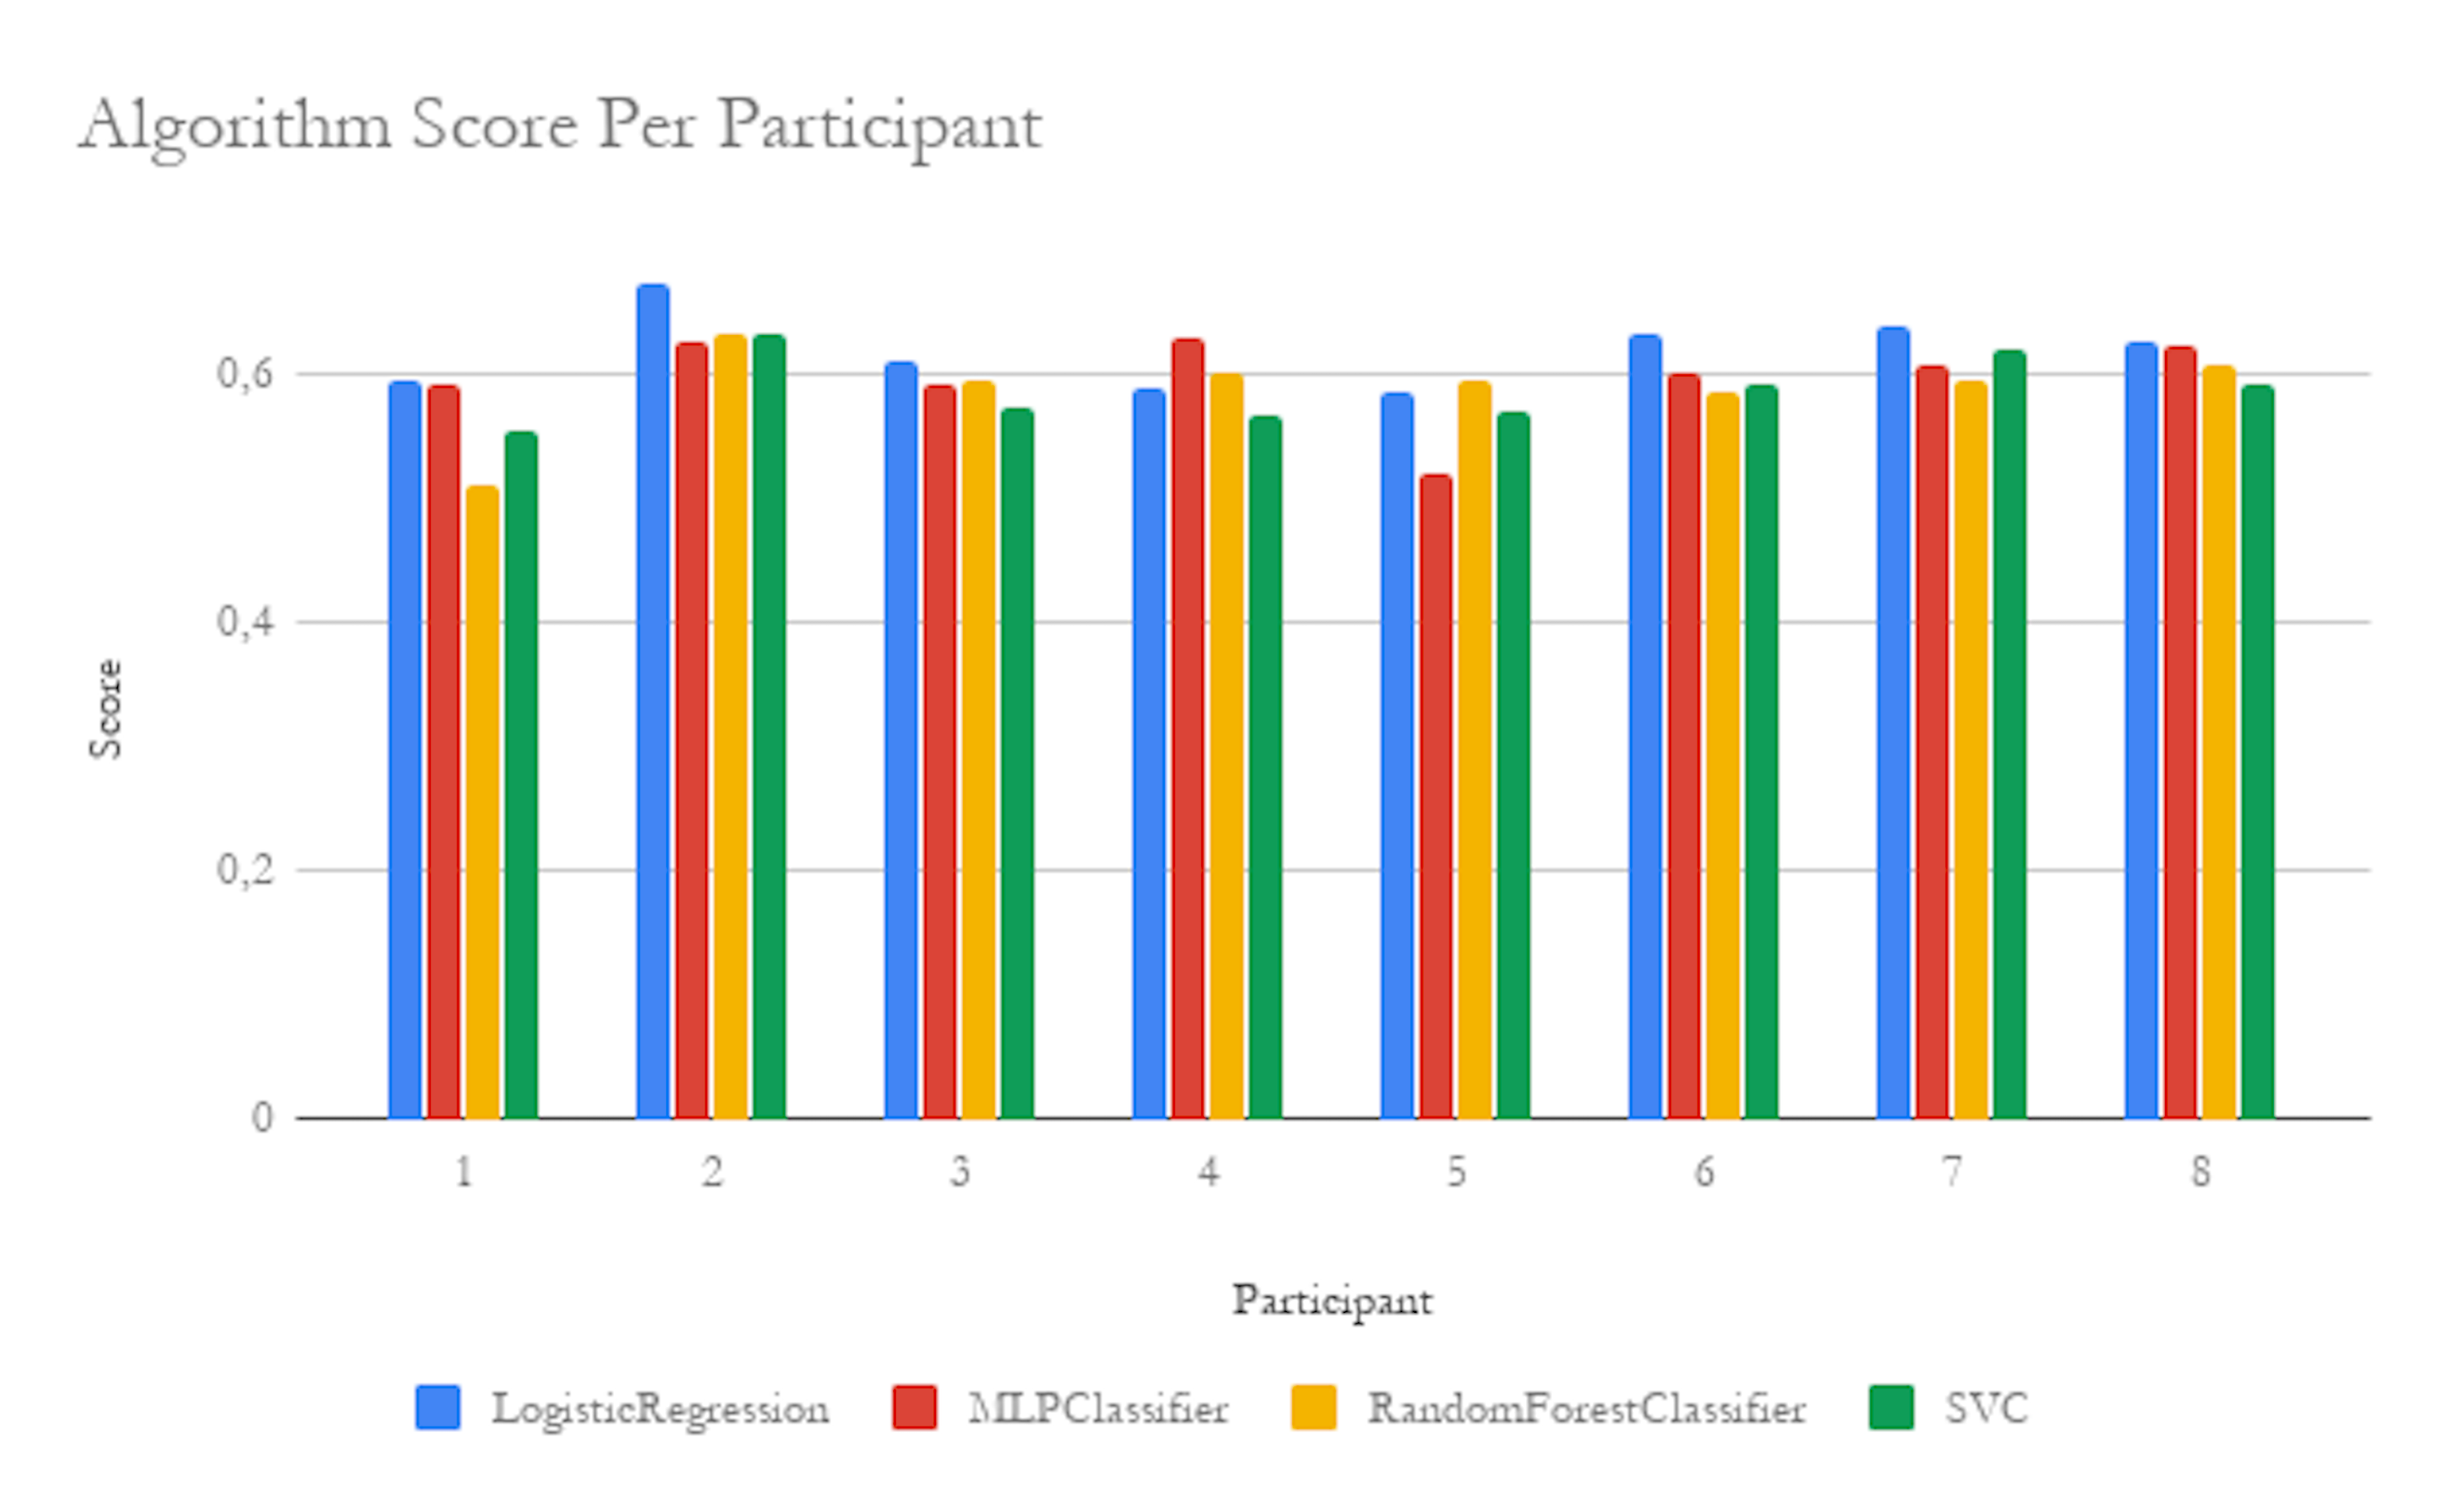
\includegraphics[scale=0.4]{Images/algorithm_calibration/Total_calib.png}
    \caption{Binary classification score using different classifiers while recognizing ErrP potentials for the eight subjects.  Chance Level is 0.5.}
    \label{fig:classifiers}
\end{figure}

\begin{figure}[ht]
    \centering
    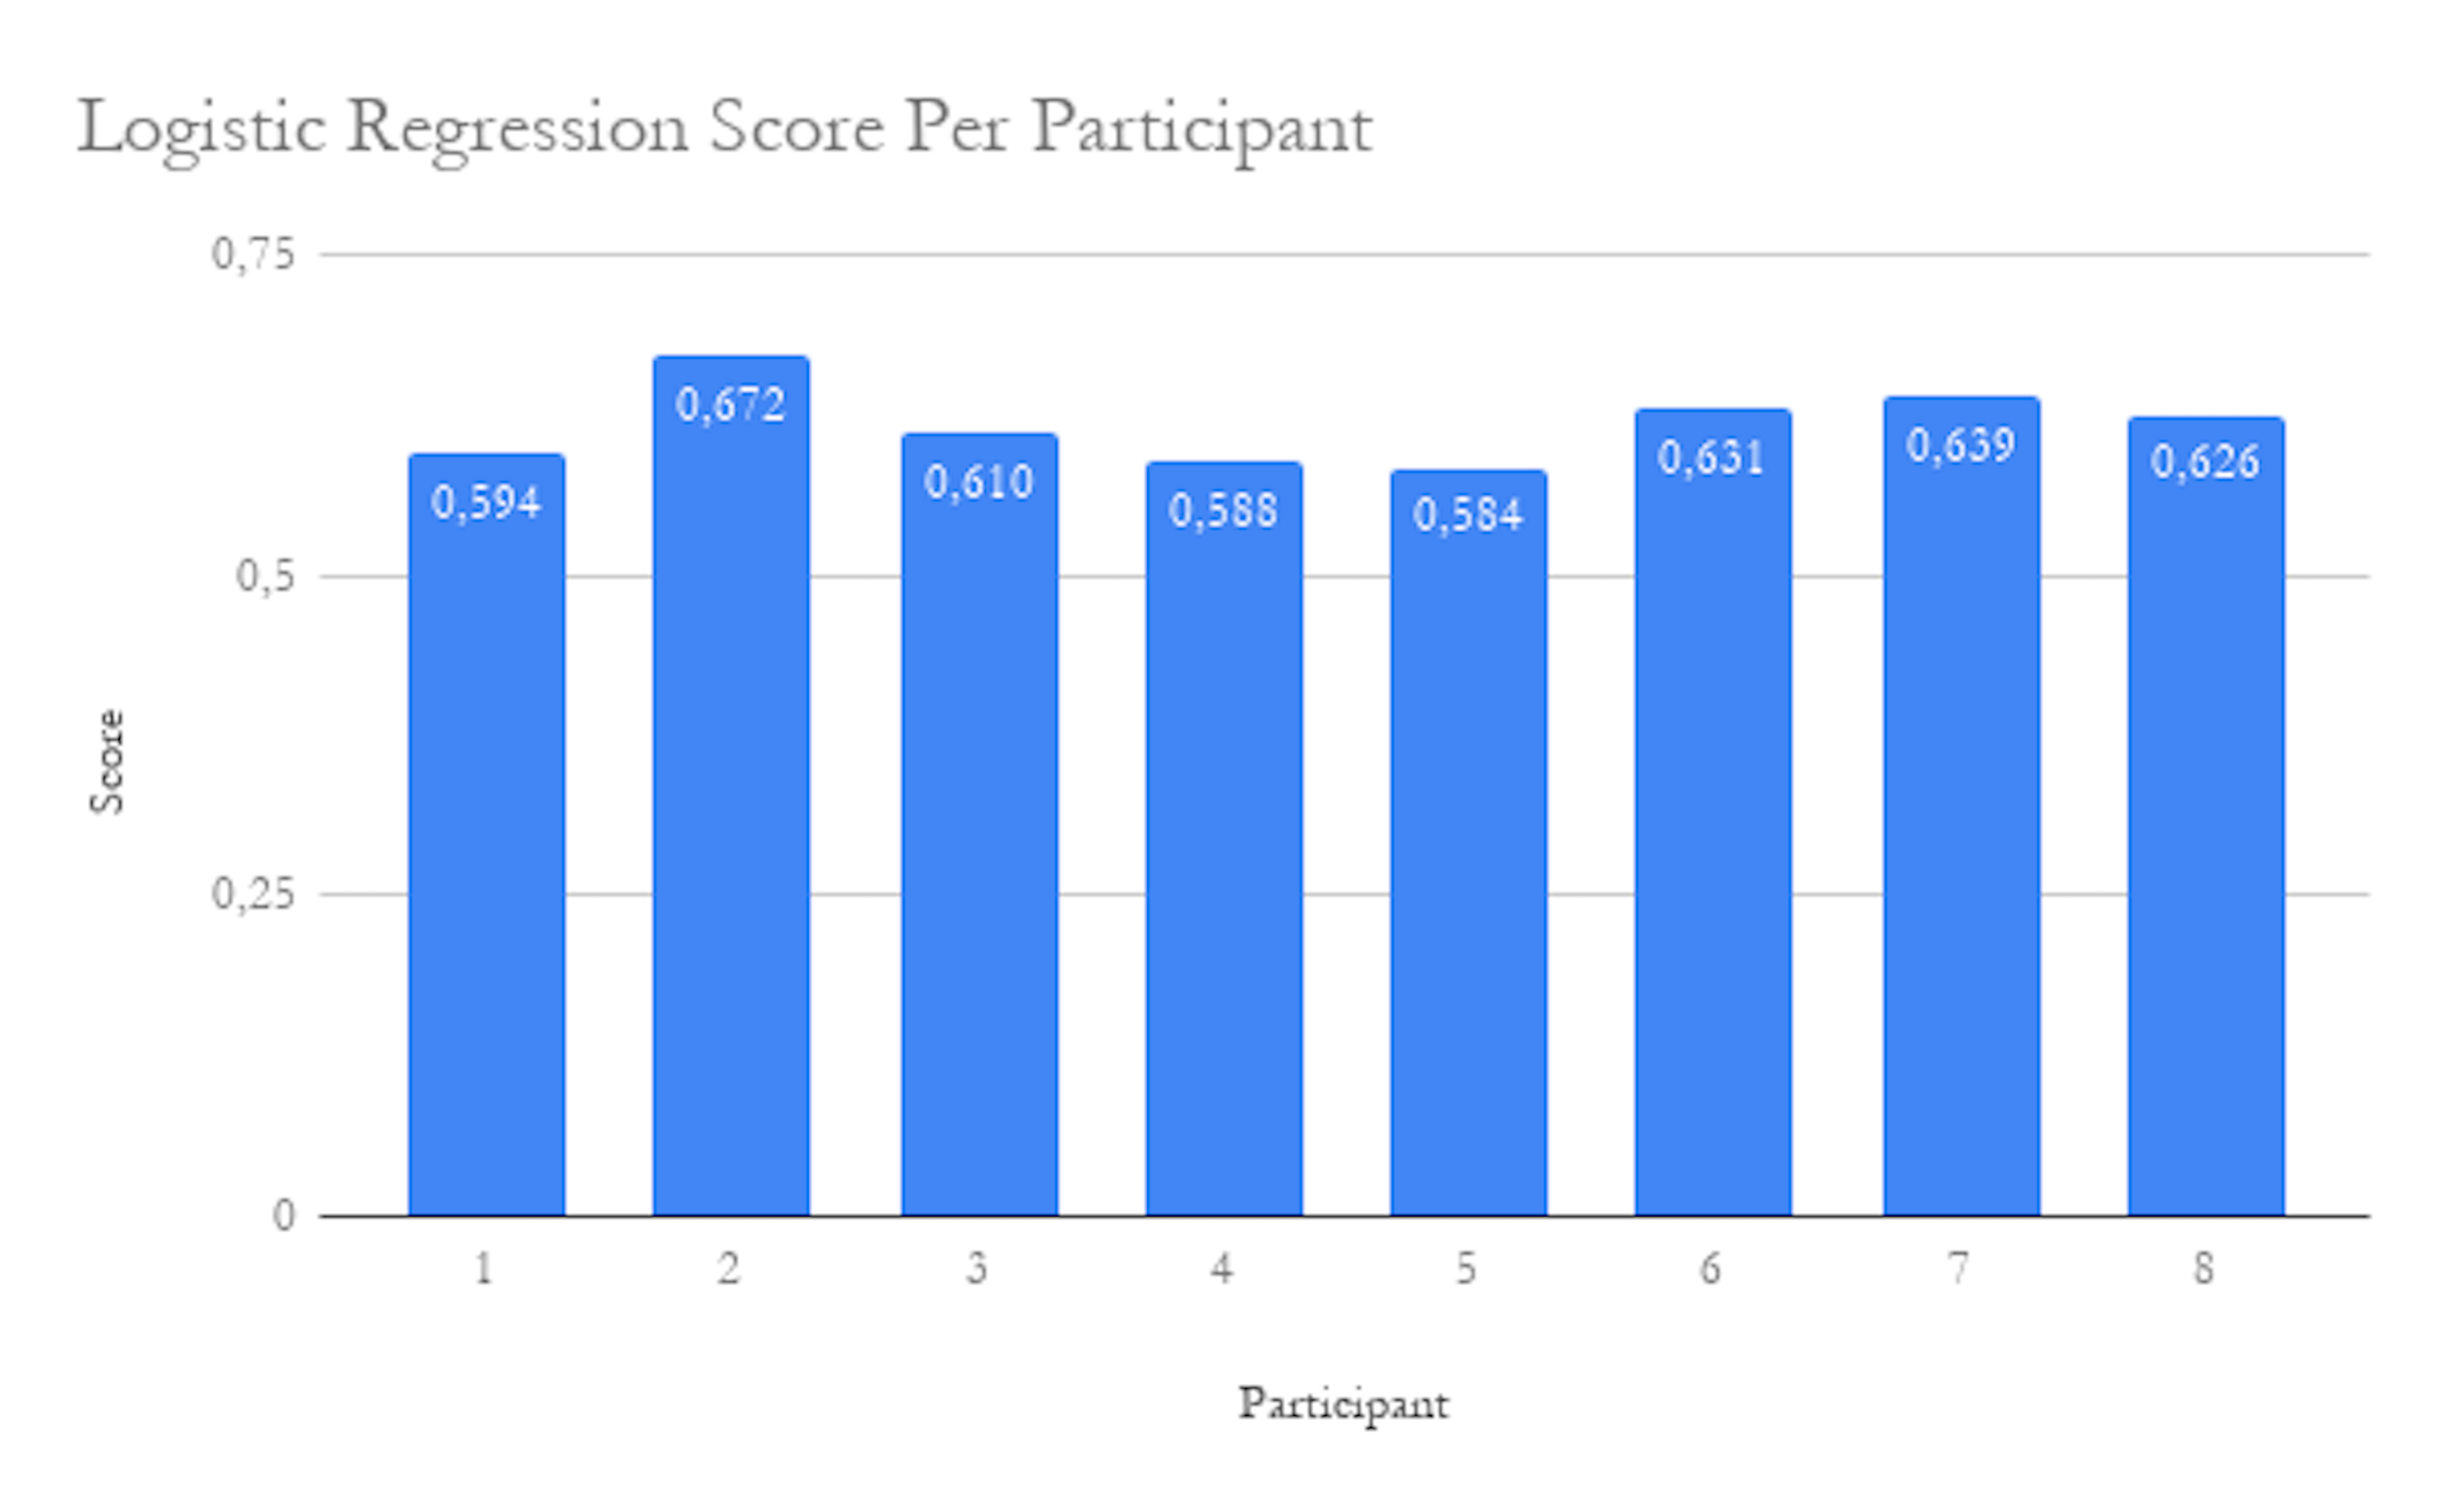
\includegraphics[scale=0.4]{Images/algorithm_calibration/LR_calib.png}
    \caption{Binary Classification Score using Logistic Regression for the eight subjects.}
    \label{fig:logisticregression}
\end{figure}

On the other hand, Figure \ref{fig:avg_steps} shows for each subject the average amount of steps the agent takes to reach the goal as the Q-Table is progressively trained using the reward information obtained from their classified experiences. Each point corresponds to the average number of steps in 200 repetitions that it takes for the agent to reach the goal for a specific Q-Table. The first point represents the amount of steps the agent takes to reach the goal for a Q-Table that hasn't been trained at all, where movements are decided randomly. The next point corresponds to the amount of steps it takes to reach the goal using a policy derived from a Q-Table trained with one experience, and so on.

\begin{figure}[h!]
\begin{subfigure}{0.5\textwidth}
\centering
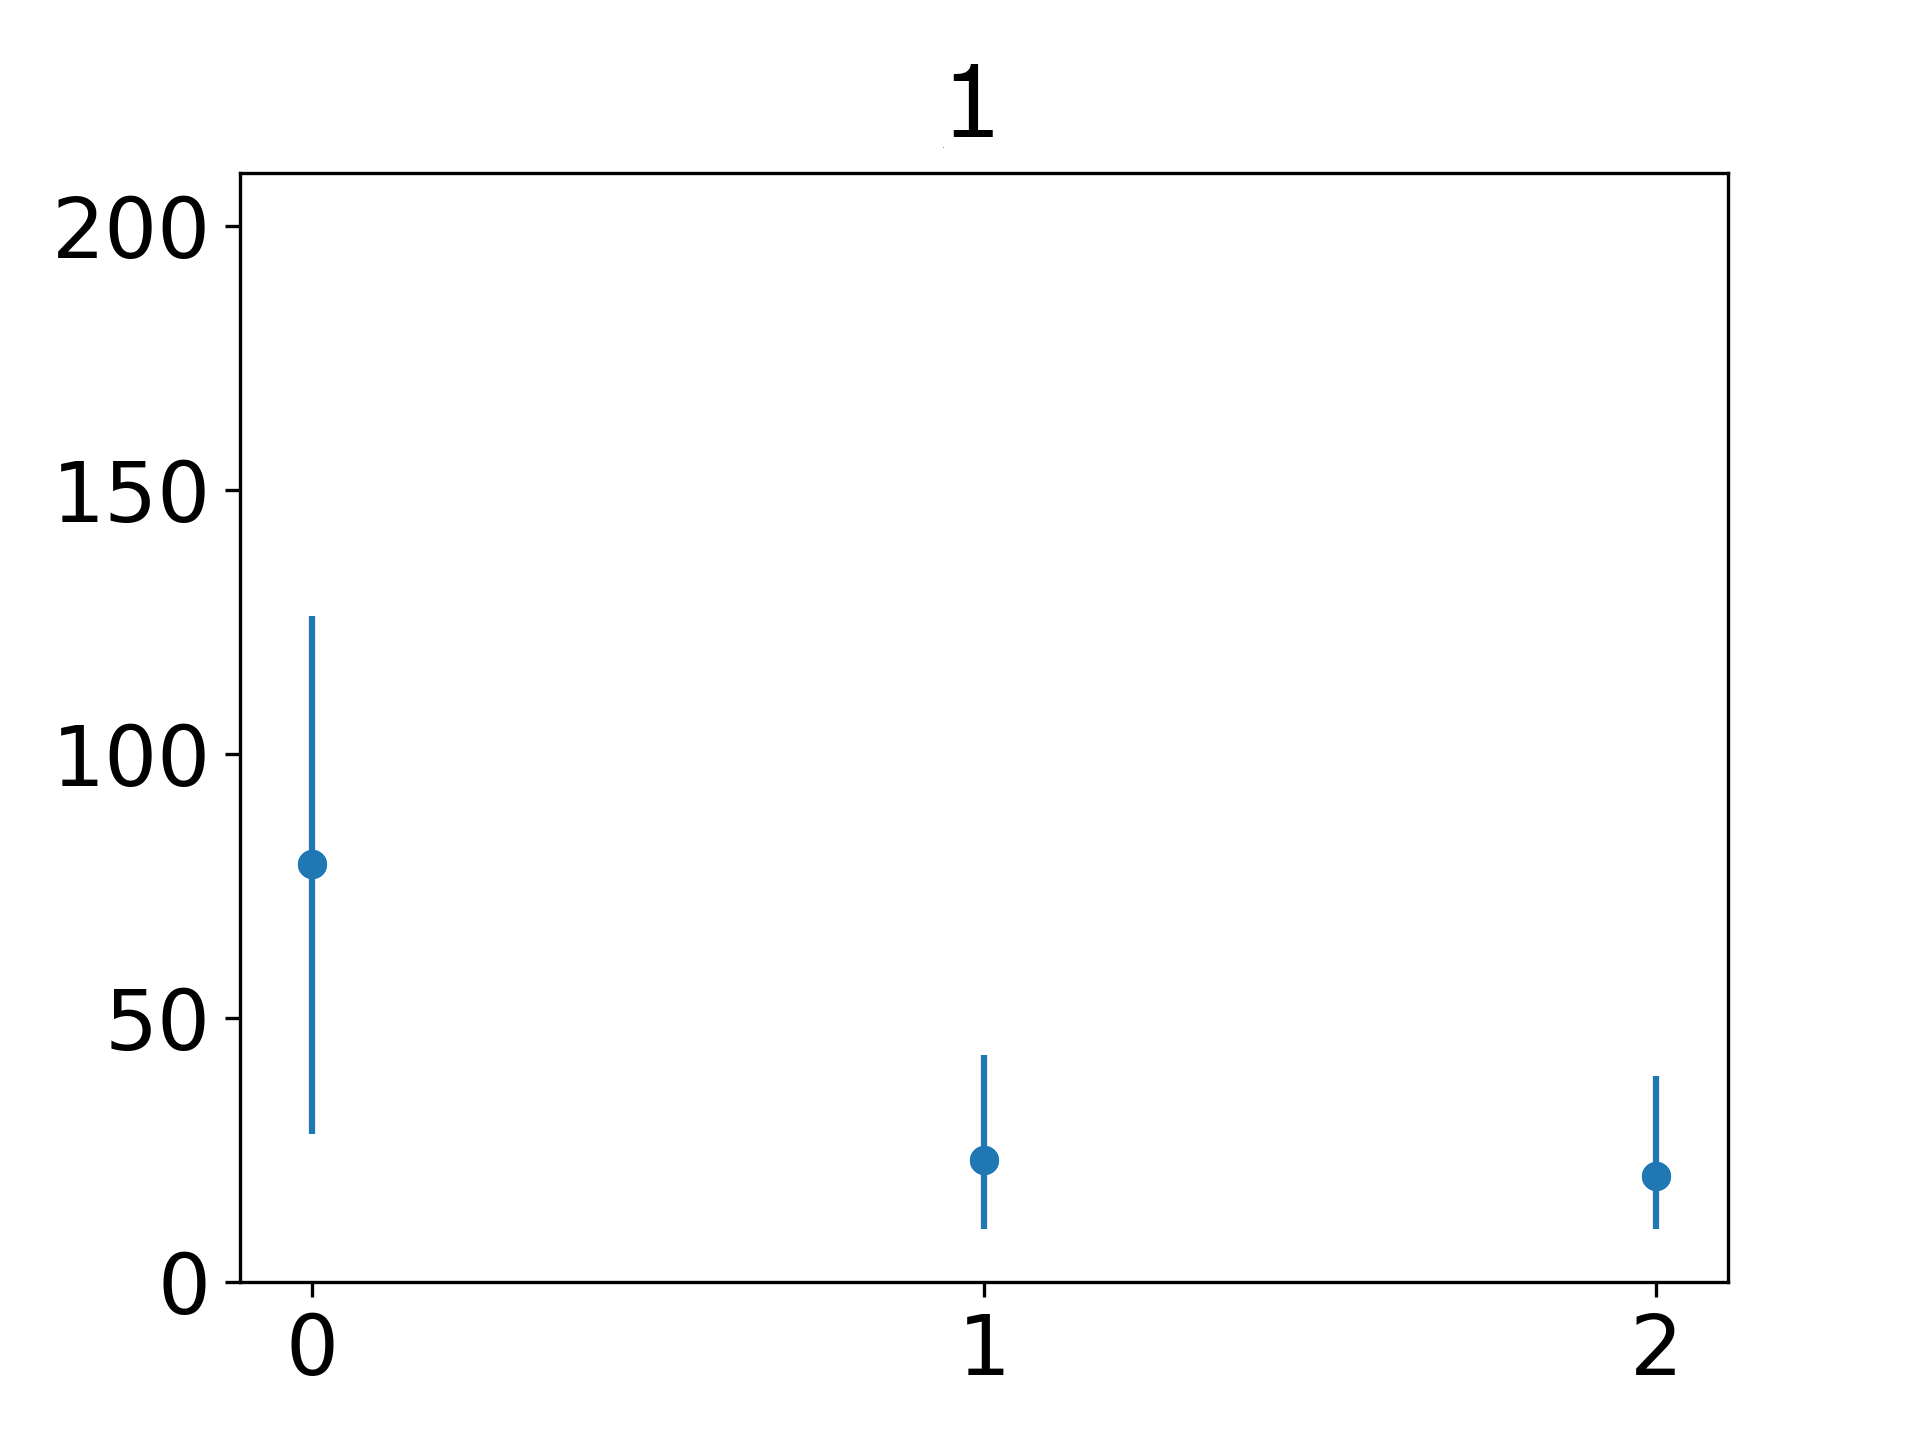
\includegraphics[scale=0.27]{Images/Average_steps/a.png}
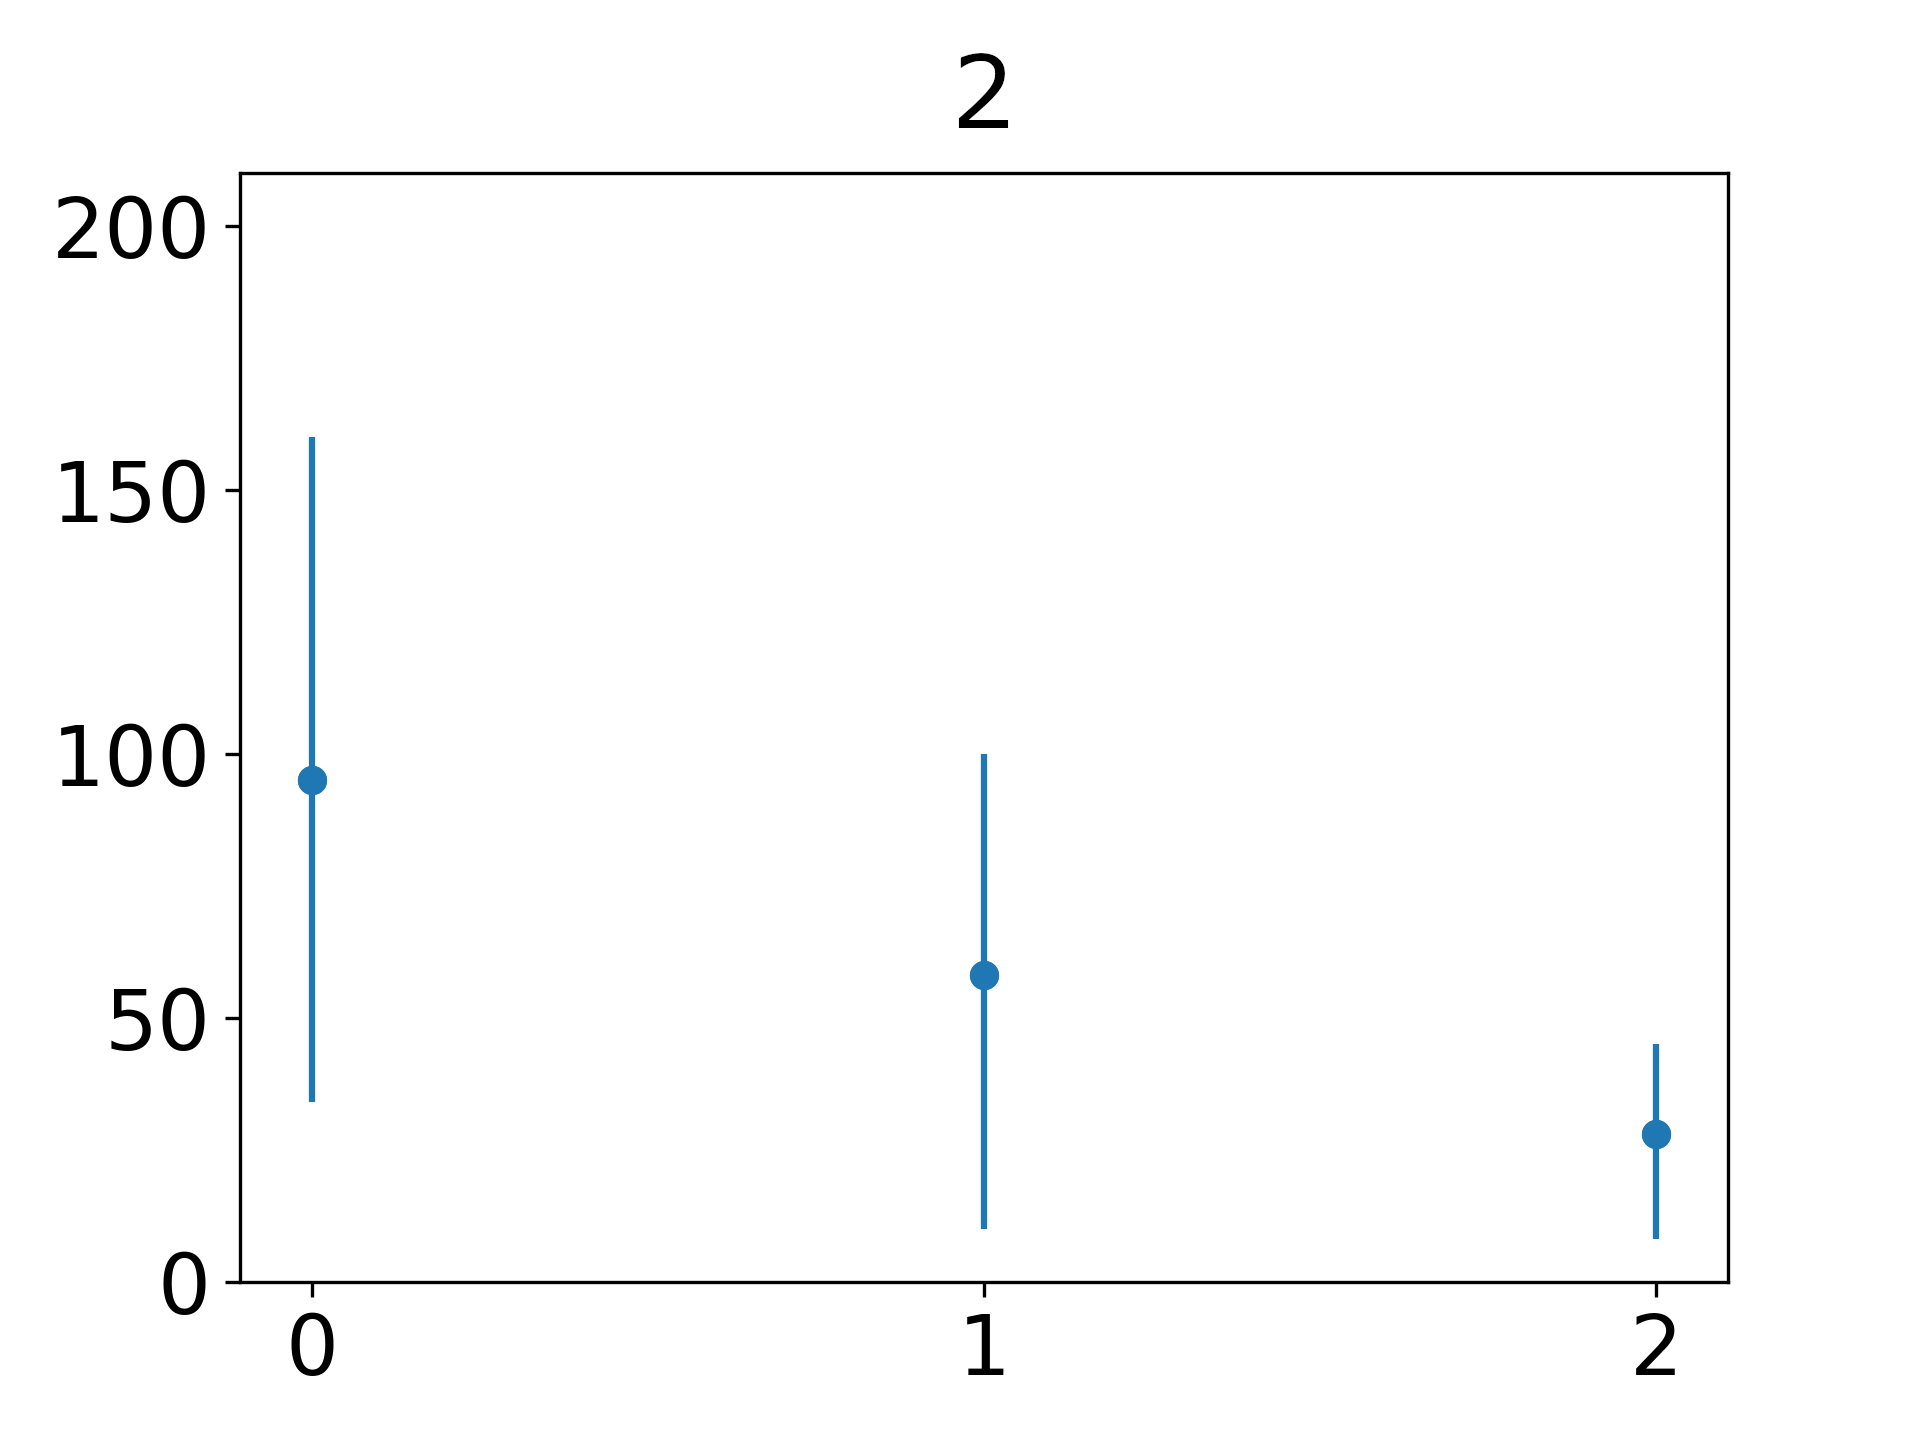
\includegraphics[scale=0.27]{Images/Average_steps/b.png}
\centering
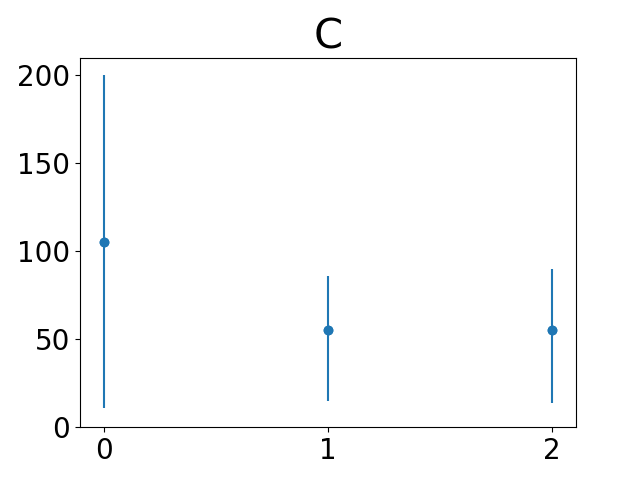
\includegraphics[scale=0.27]{Images/Average_steps/c.png}
 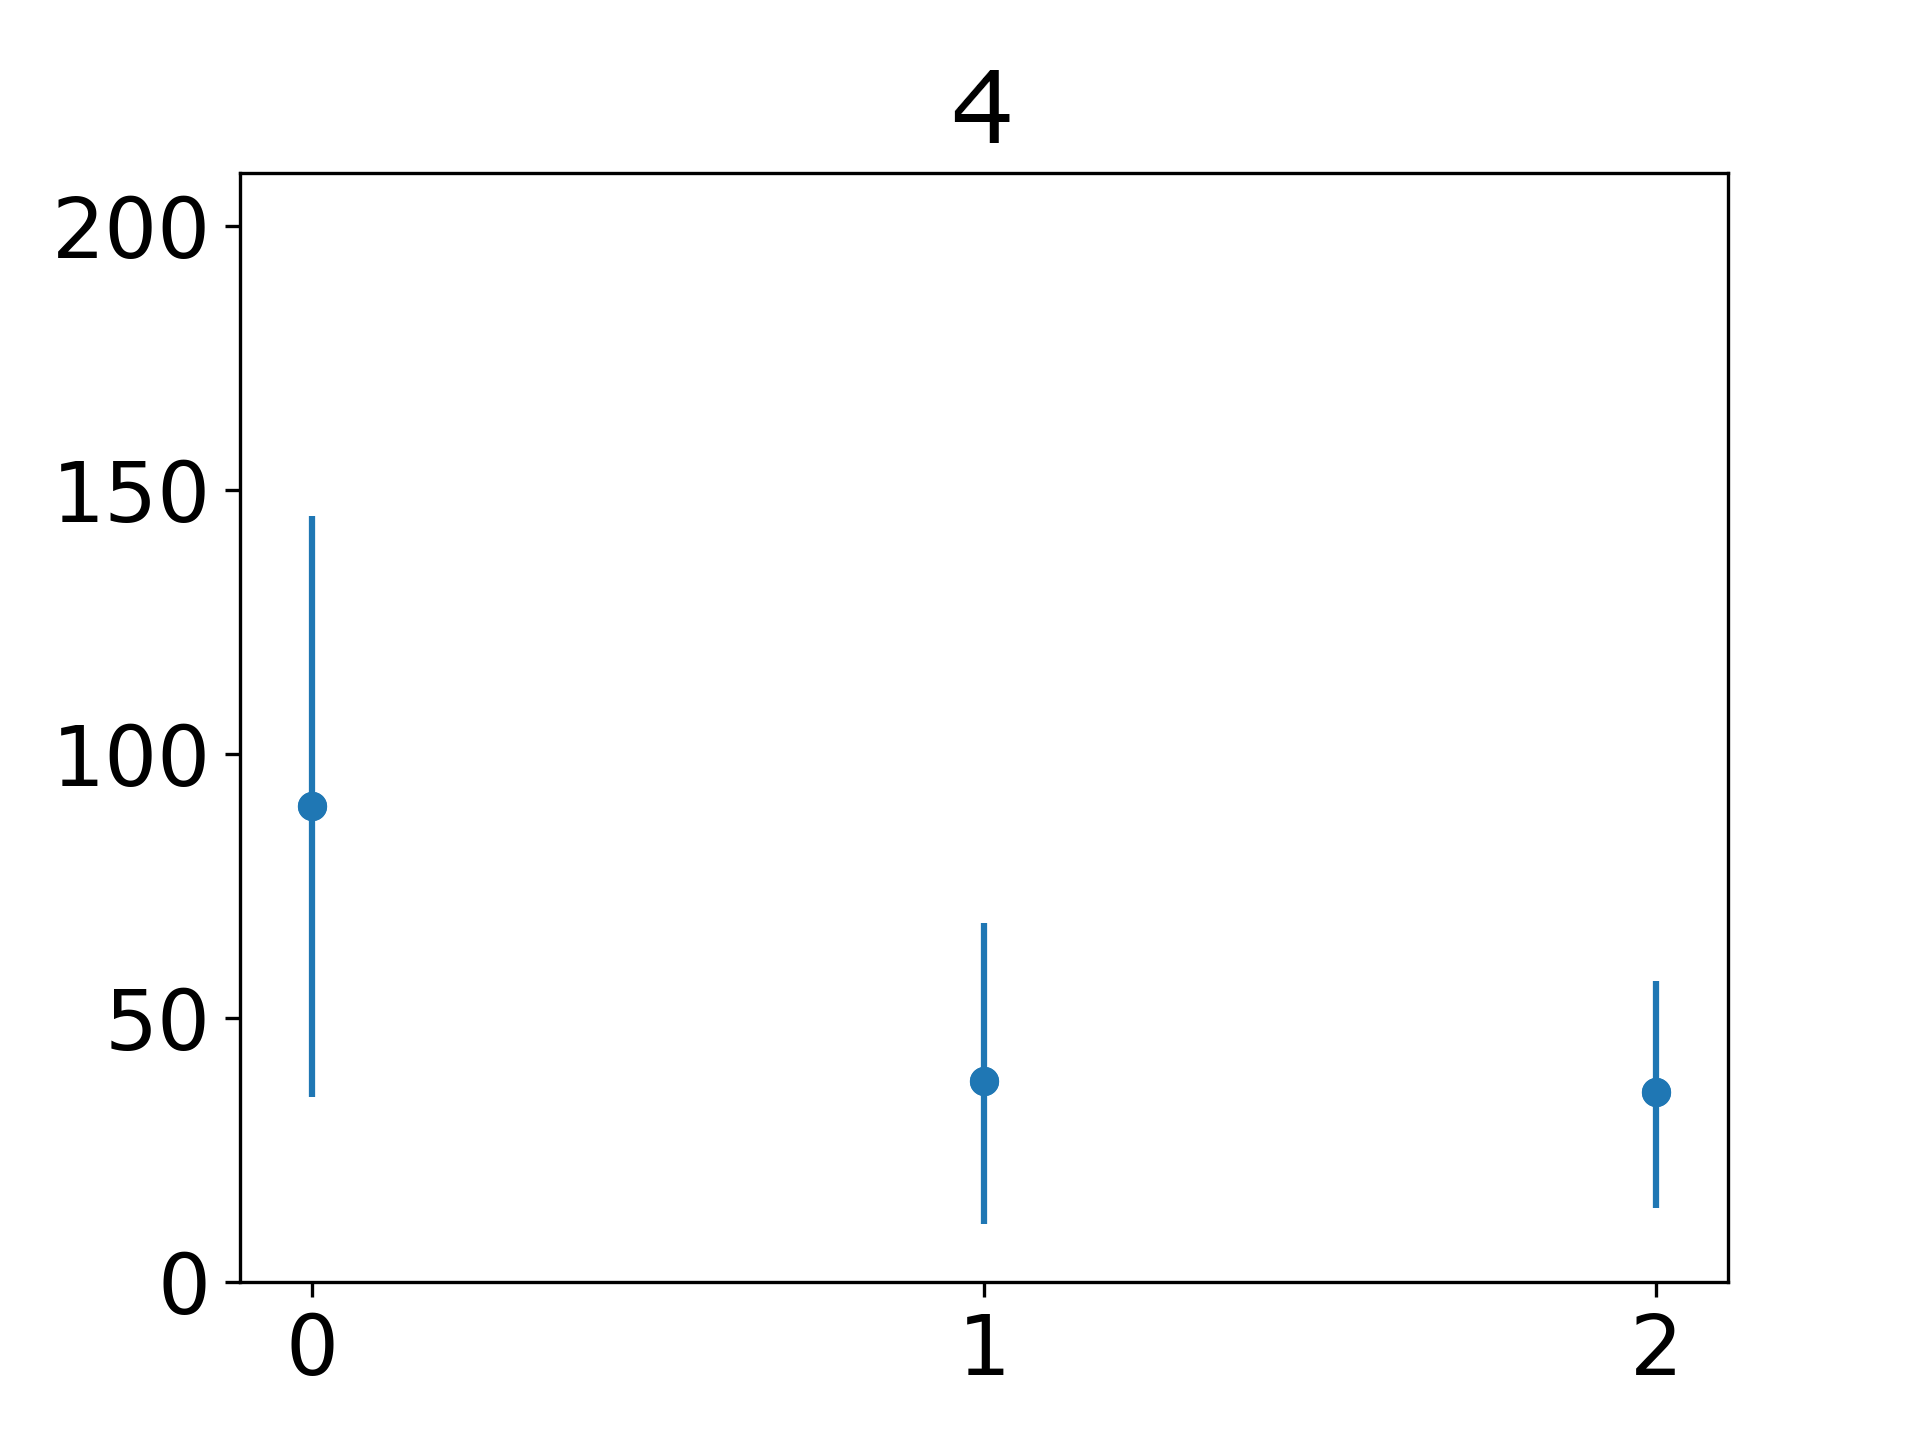
\includegraphics[scale=0.27]{Images/Average_steps/d.png} 
 \centering
  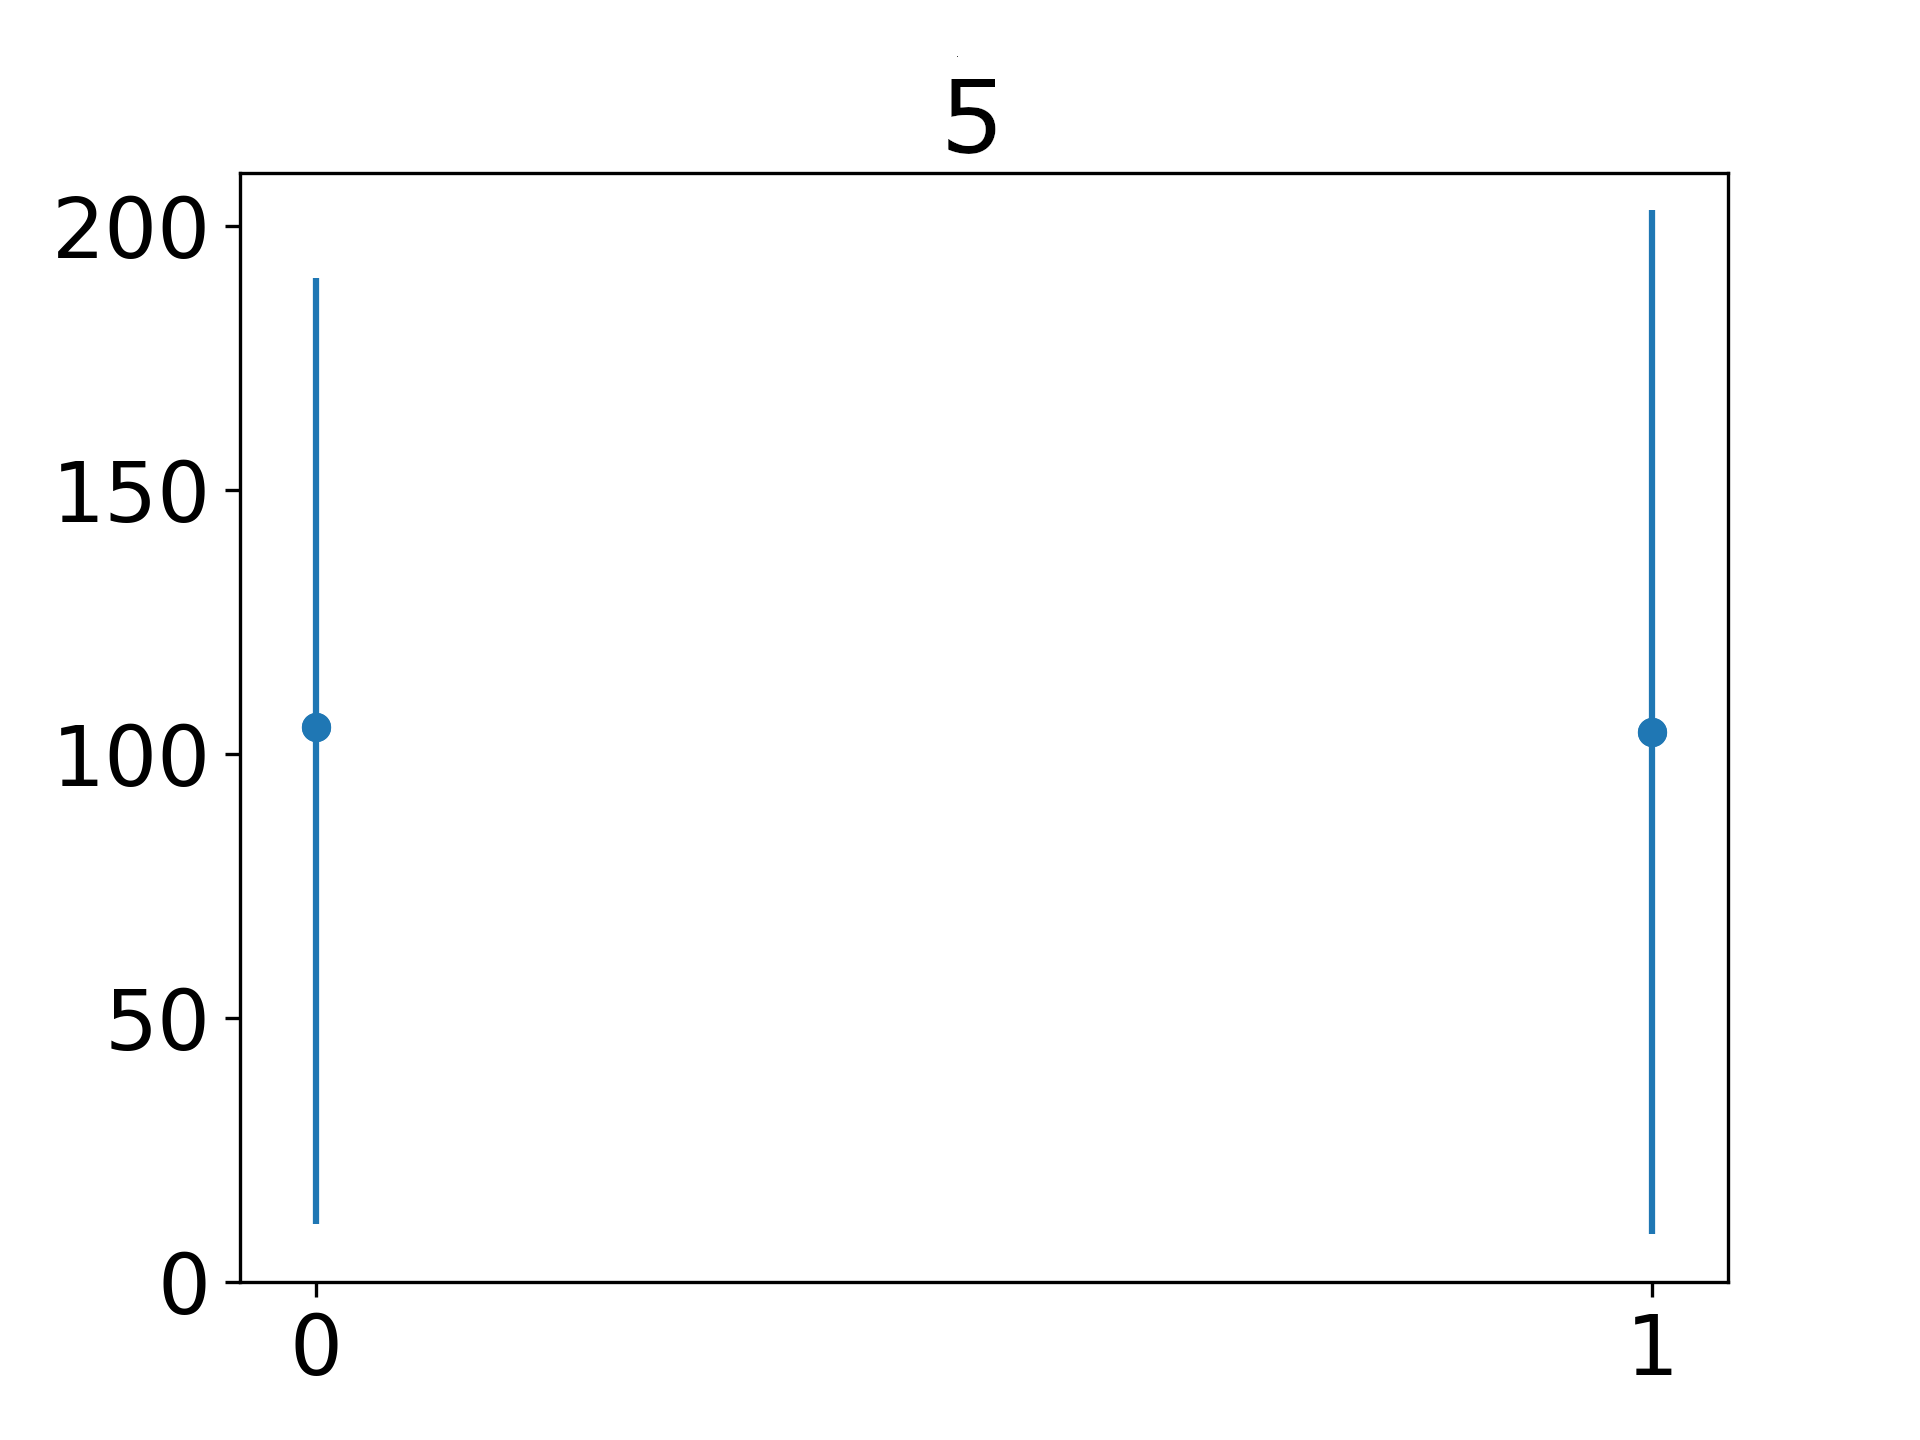
\includegraphics[scale=0.27]{Images/Average_steps/e.png} 
  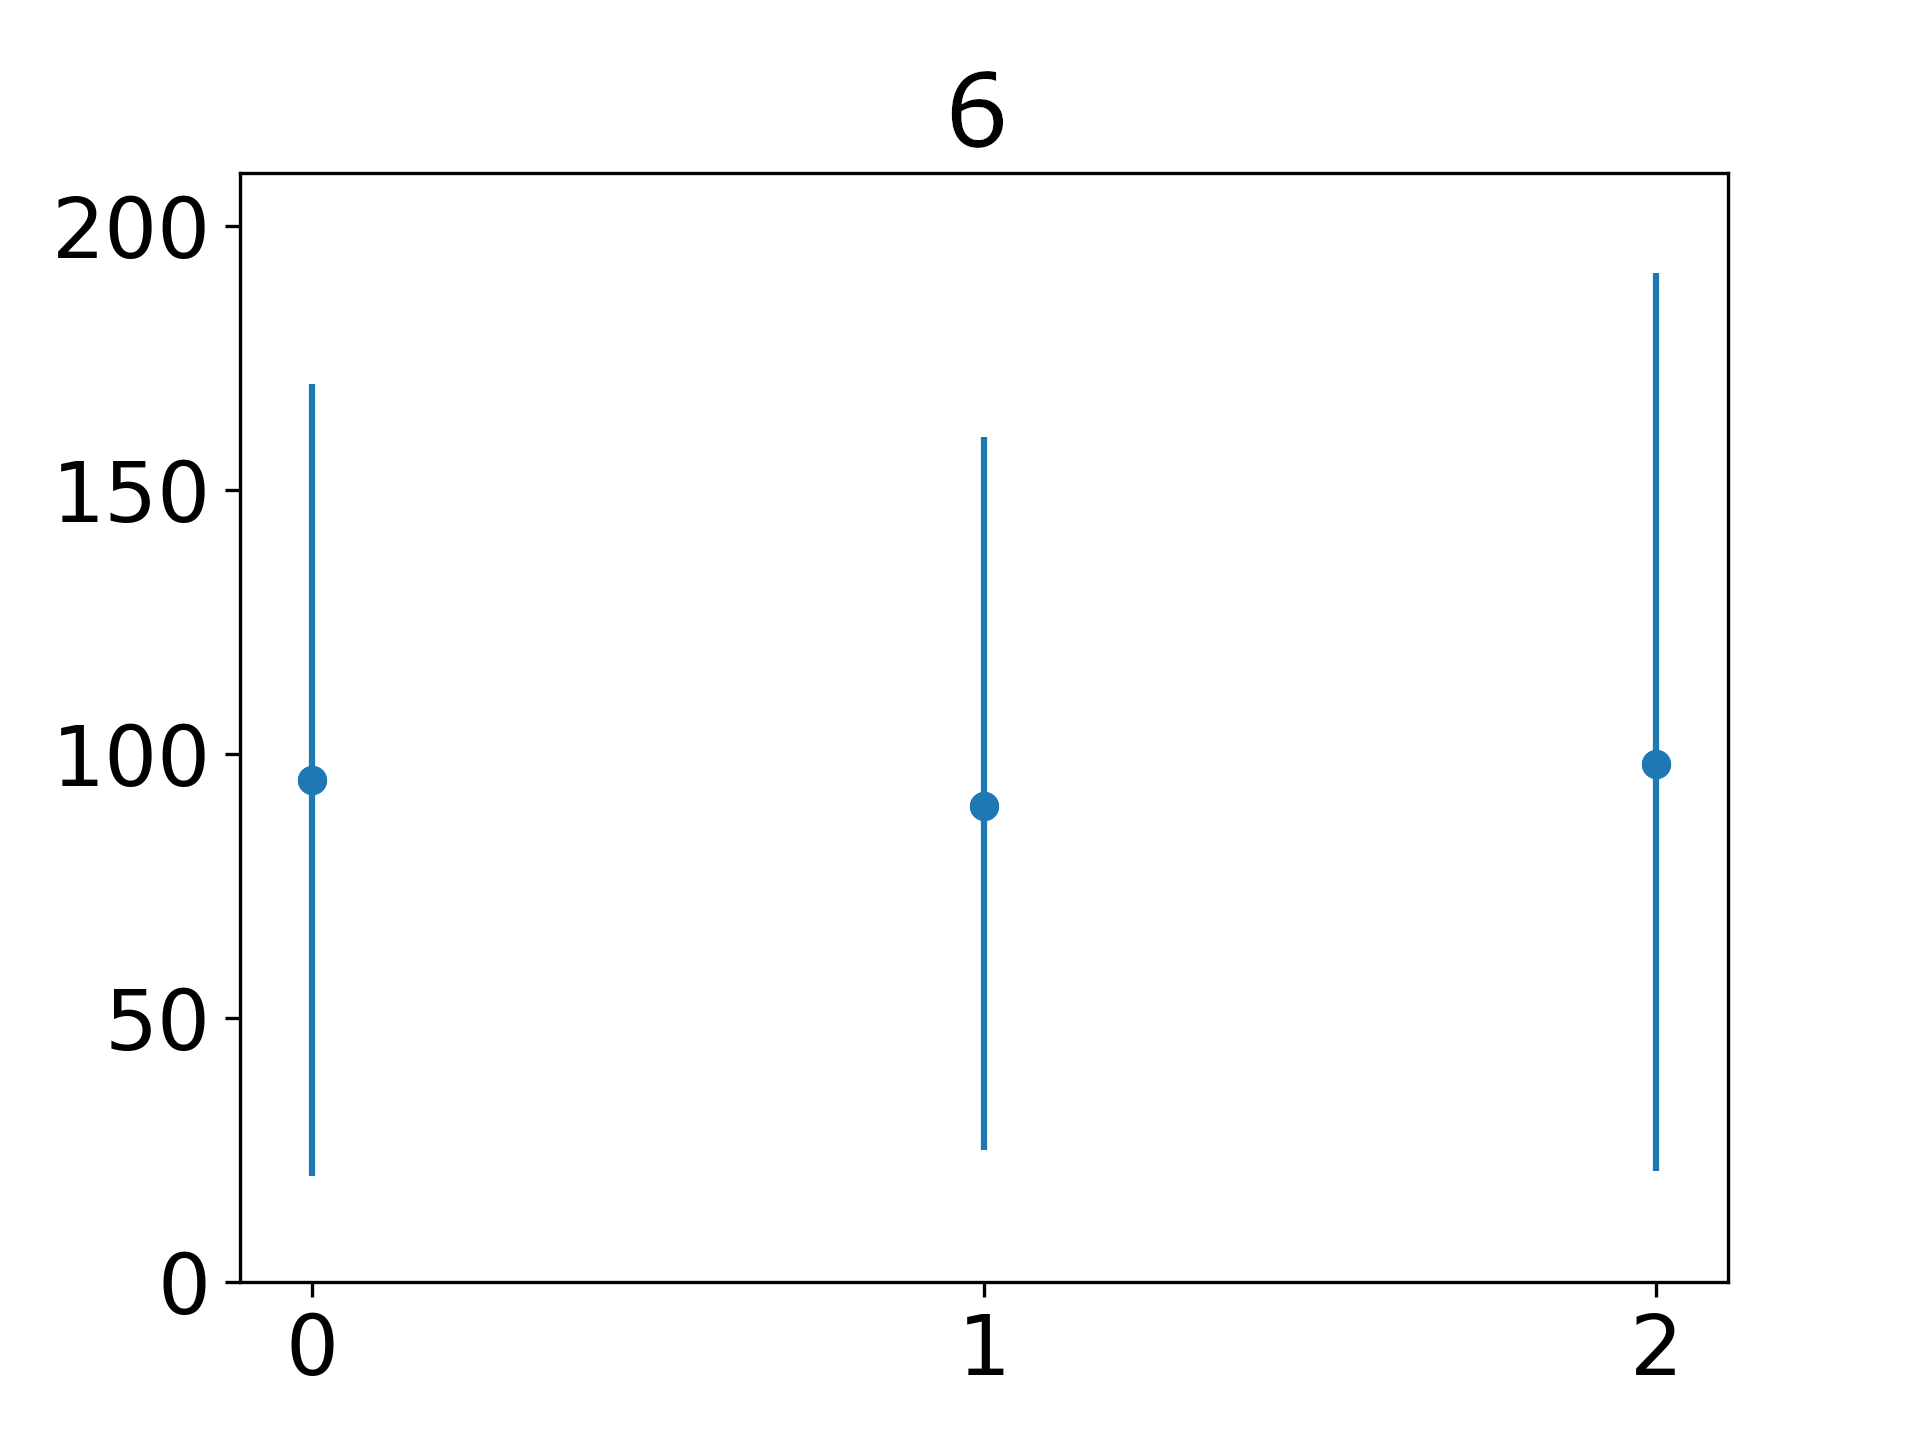
\includegraphics[scale=0.27]{Images/Average_steps/f.png} 
  \centering
  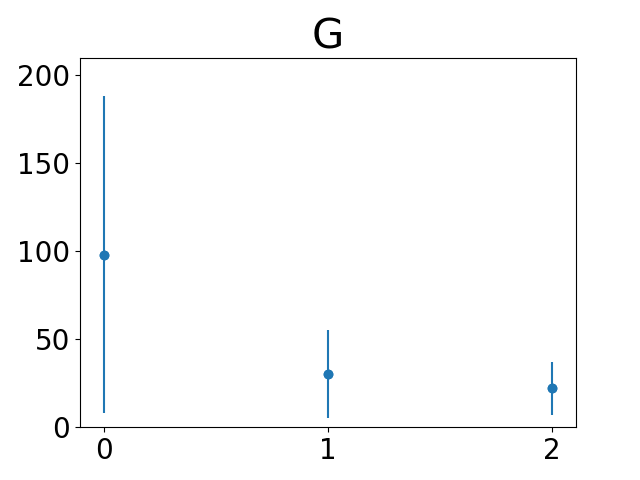
\includegraphics[scale=0.27]{Images/Average_steps/g.png} 
  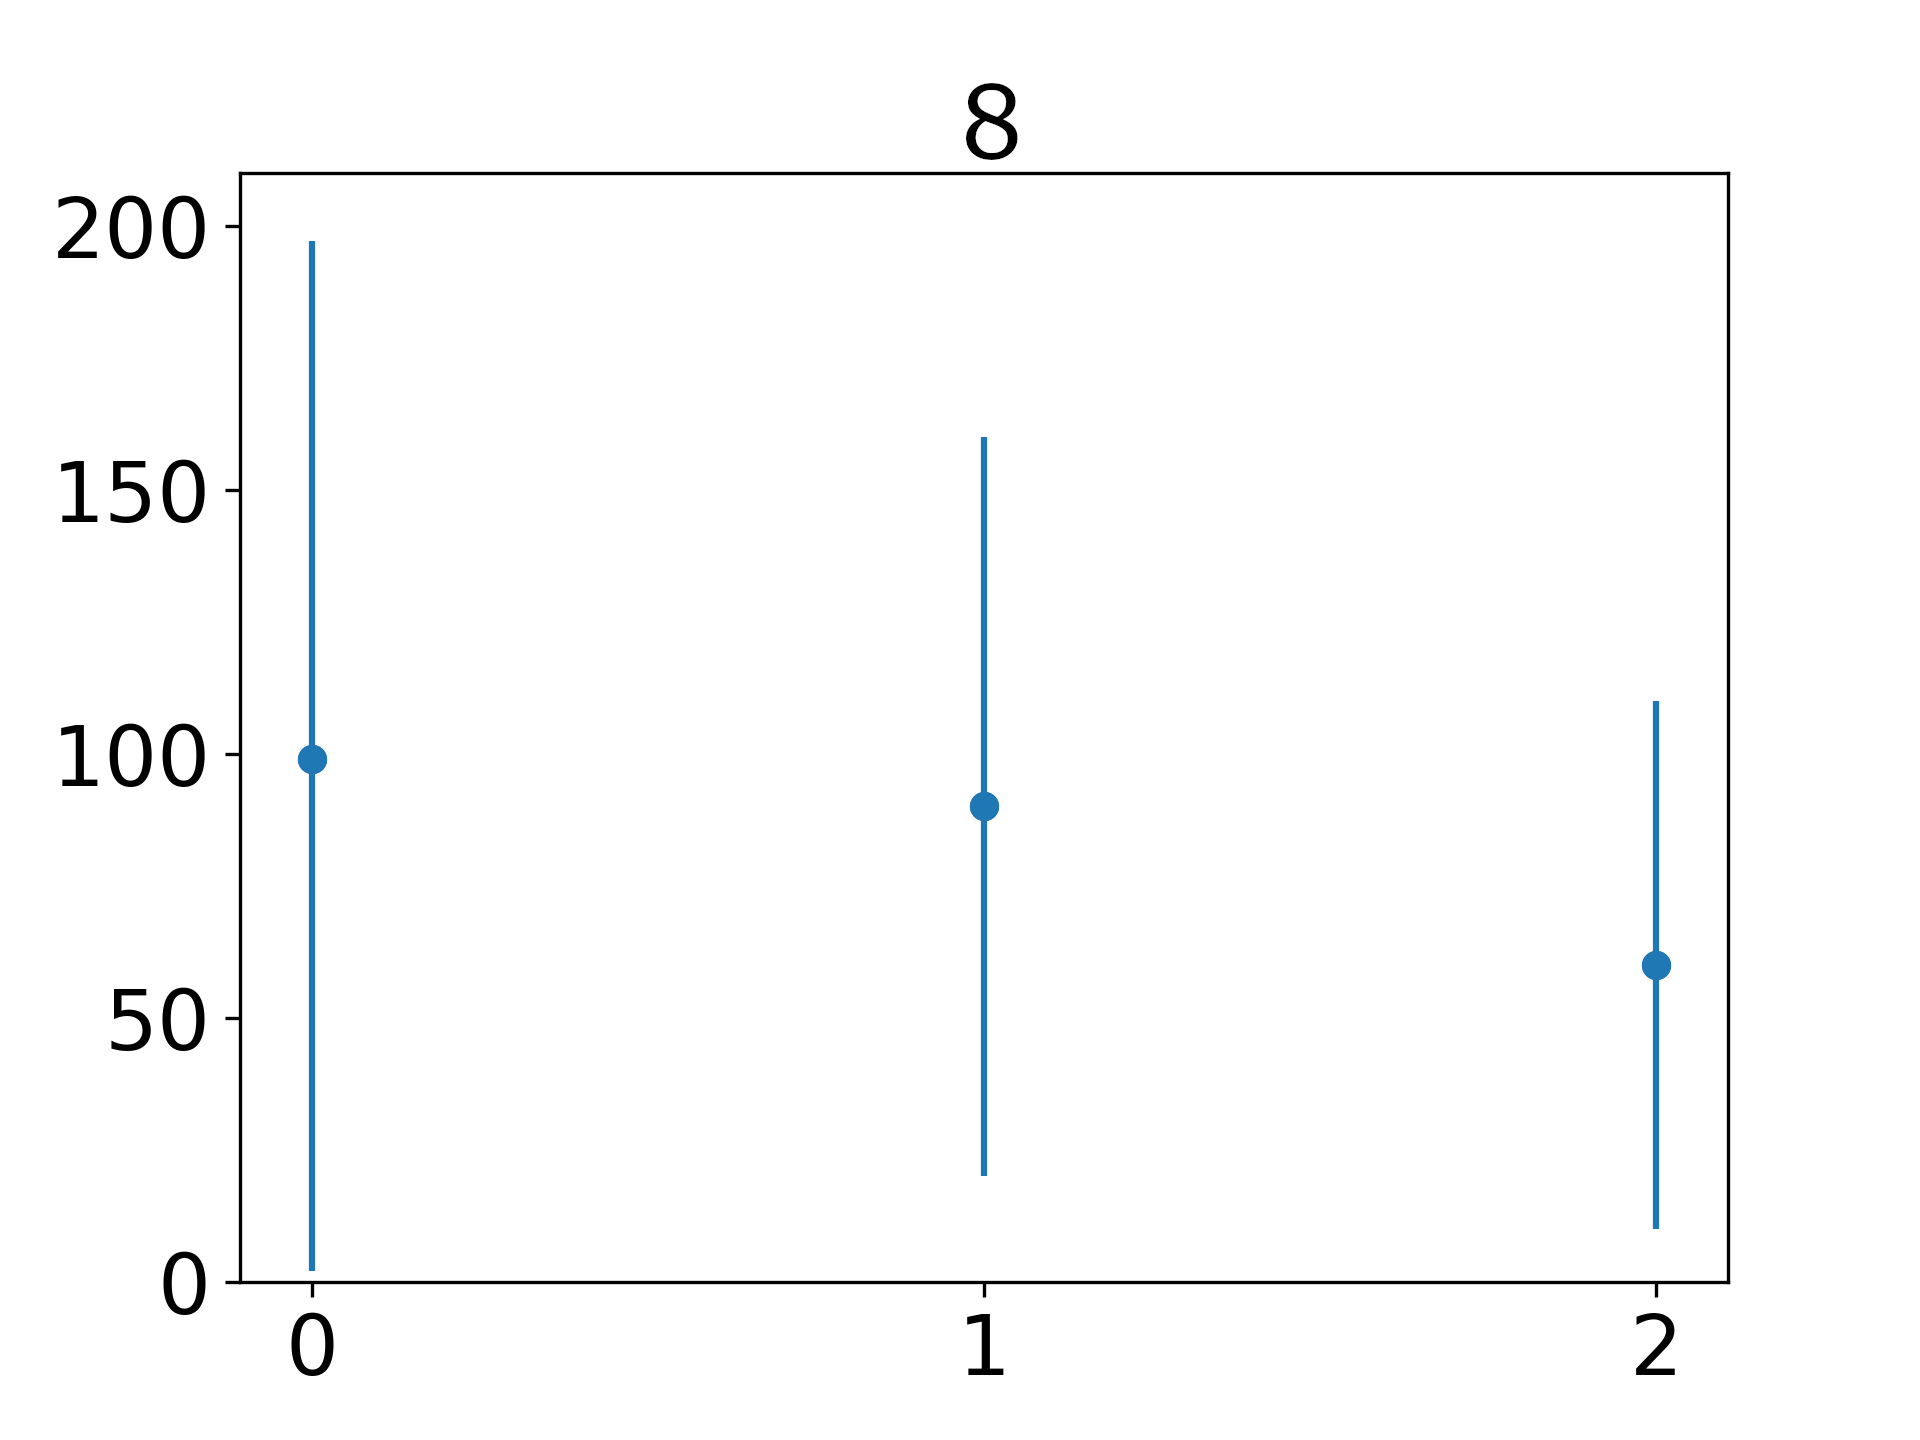
\includegraphics[scale=0.27]{Images/Average_steps/h.png} 
\end{subfigure}
\caption{Average number of steps for the agent when trained with experiences from subjects 1-8. Y axis show the averaged number of steps, while x axis show the number of experiences used to cumulative train the Q-Table.}
\label{fig:avg_steps}
\end{figure}


The results show that as the Q-Table is progressively trained the average amount of steps decreases, meaning that the agent learns. However, the rate at which it learns varies per subject, depending on the classification accuracy of the extracted brainwaves.  For example results for subject 1 show faster learning than those of subject 8 (Figure \ref{fig:avg_steps}).

In the case for subject 5 and 6, the reward information obtained from the brainwaves is not enough to train the agent effectively. Figures \ref{fig:avg_steps} E and \ref{fig:avg_steps} F show no apparent learning, as the amount of steps to reach the goal doesn't decrease when trained.  These results are also consistent with their classification ROC curves, shown on Figures~\ref{fig:rocsubjects} obtained for both subjects, where the area under the curve are close to chance level.  Both subjects have less recorded data from the sessions in comparison to the rest of the subjects.   This variation in performance for different subjects has been studied extensively in BCI.  Besides low data samples there are other reasons affecting the classification accuracy:  cognitive reasons, this being the subject not paying extensively attention to the game dynamics, very low Signal-To-Noise Ratio (SNR) of the ErrP component or even the BCI-illiteracy phenomena where the specific subject's signals do not contain the expected component response~\cite{Yousefi2019}.

\begin{figure}[h!]
\captionsetup[subfigure]{justification=centering}
\begin{subfigure}{0.25\textwidth}
    \centering
    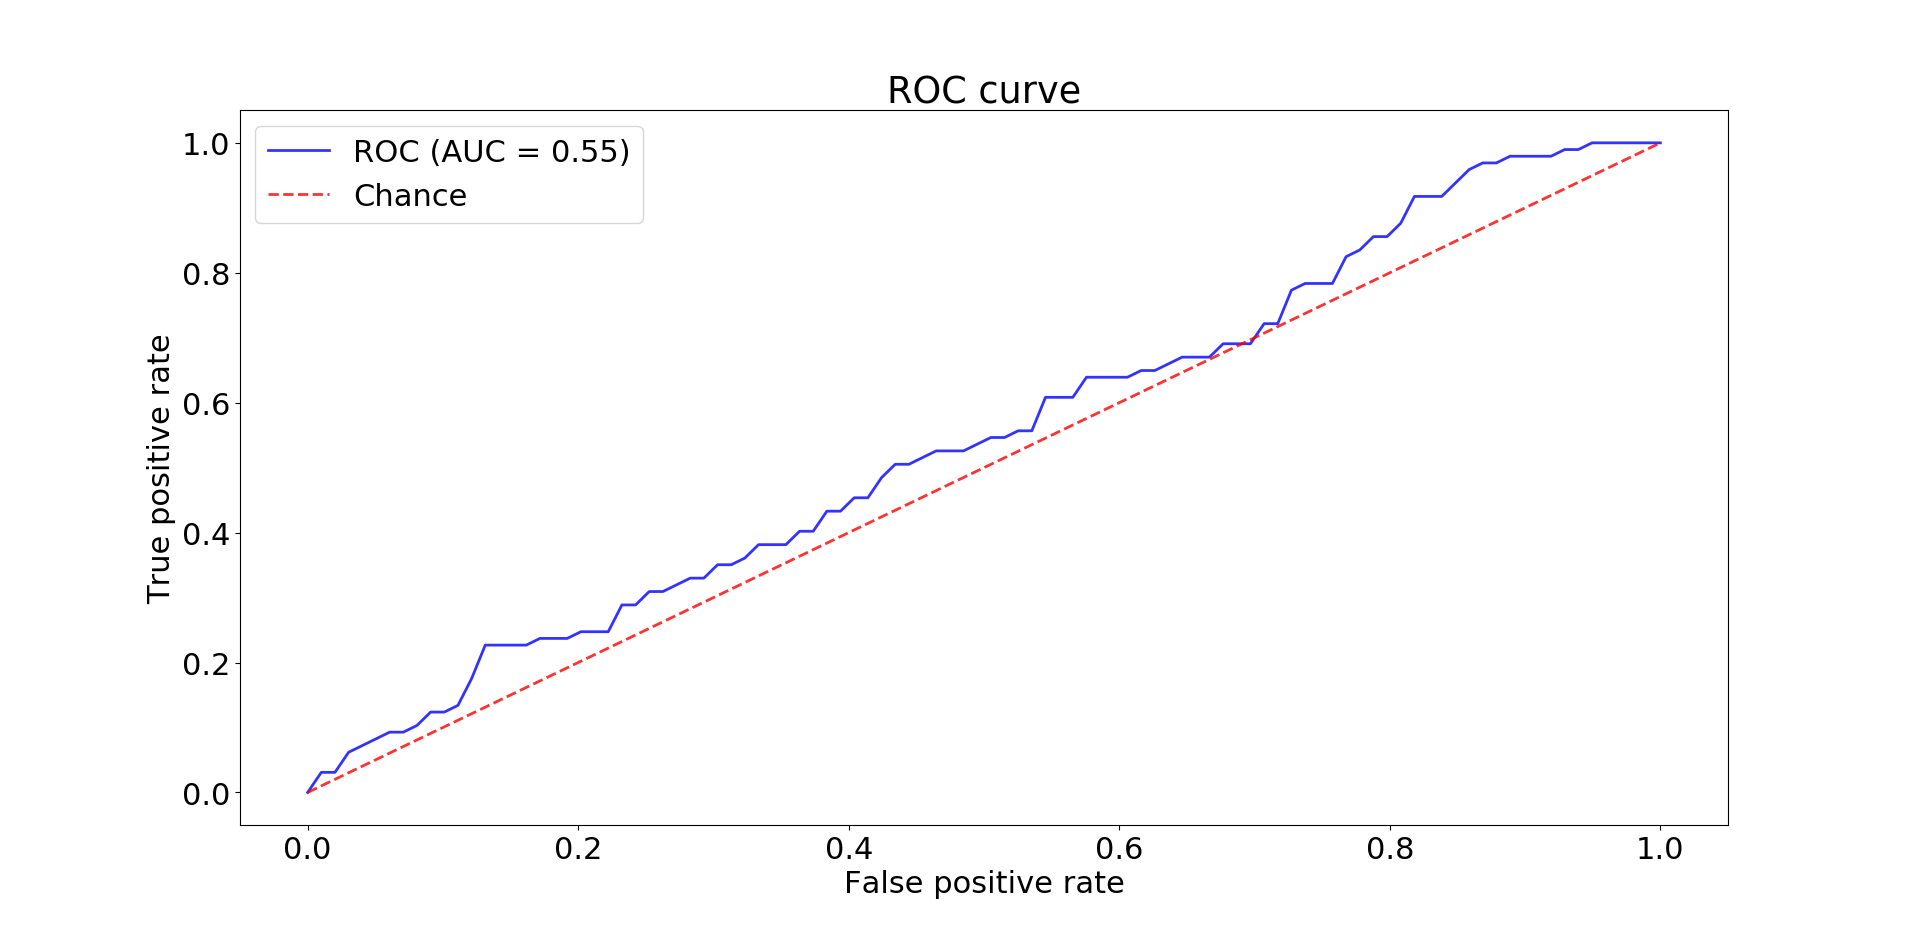
\includegraphics[scale=0.2]{Images/Classification_test/roc_e.png}
\end{subfigure}
\begin{subfigure}{0.25\textwidth}
    \centering
    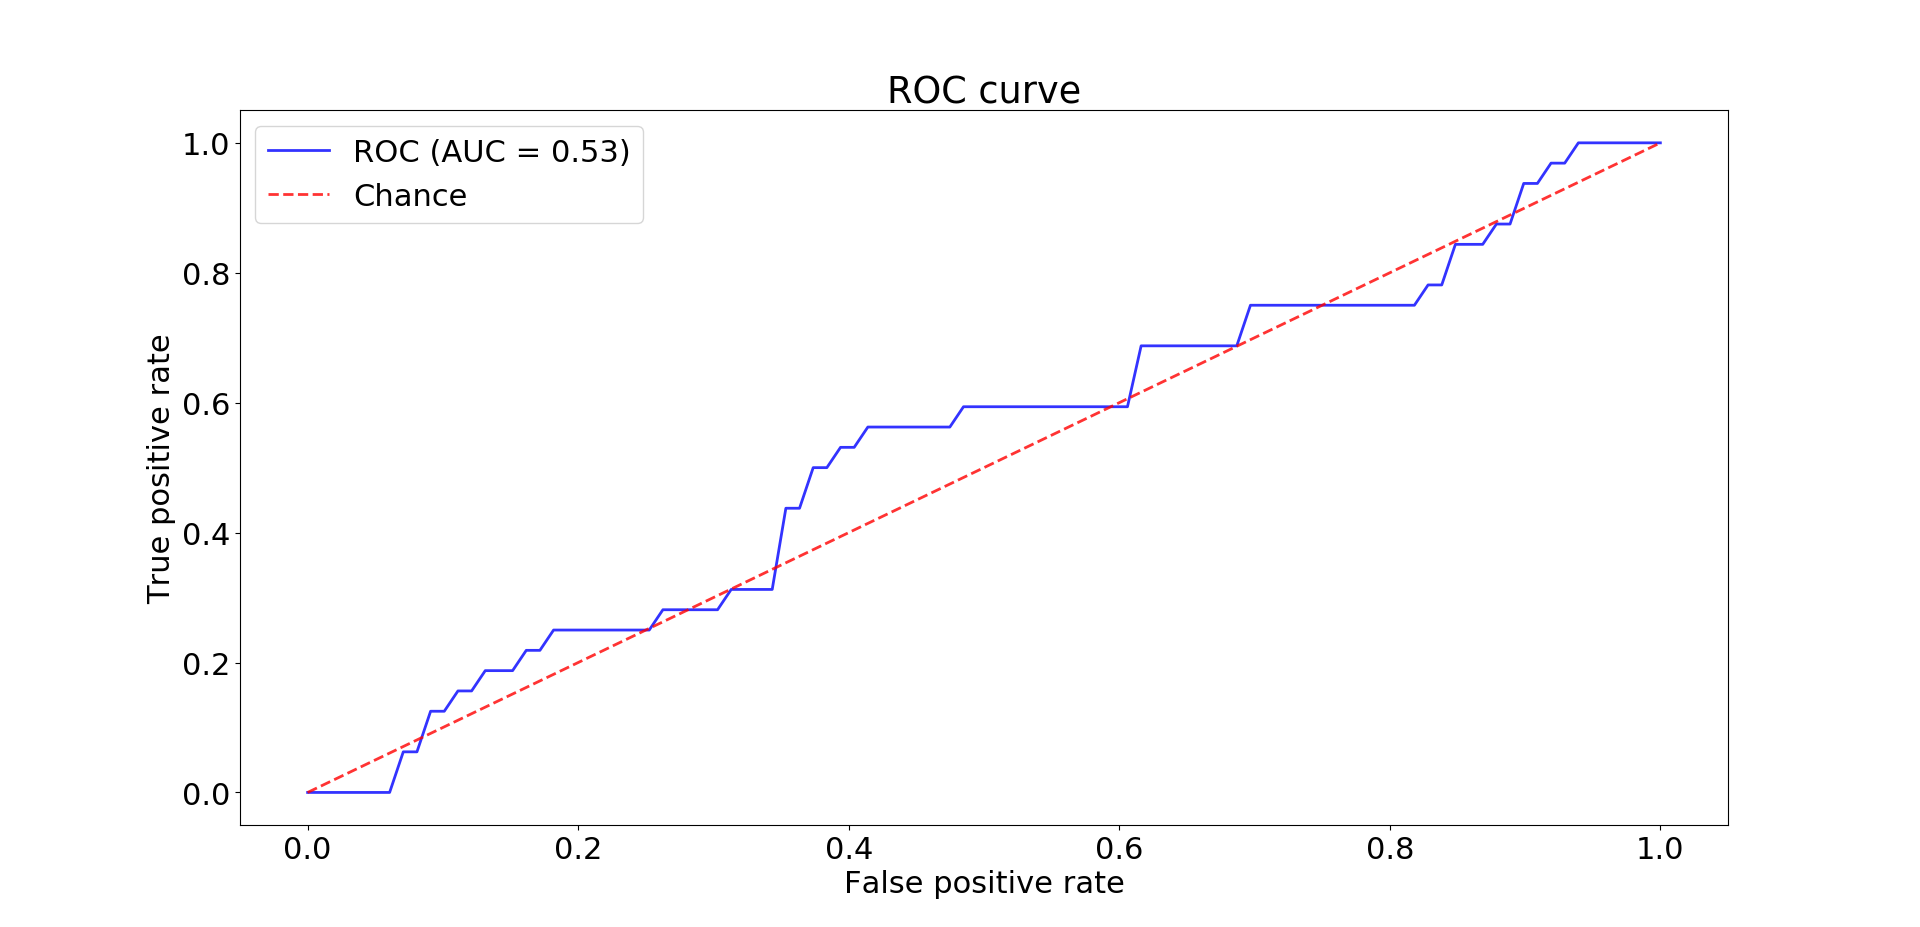
\includegraphics[scale=0.2]{Images/Classification_test/roc_f.png}  
\end{subfigure}
\caption{ROC Curves for subjects 5 (up) and 6 (down)}
\label{fig:rocsubjects}
\end{figure}

%These results are consistent with fig. \ref{fig:roc:e} and fig. \ref{fig:roc:f}, which show that the signal classification for these subjects hasn't been particularly successful. 

Figure~\ref{fig:avg_steps_noise} shows the result of an agent successively trained with experiences obtained from a brainwave session, generated with sham signals.  In this case, random EEG signals were generated using OpenVibe Acquisition Server signal generator for all channels, as if they were generated from a human observer who doesn't pay attention to the game.  As it can be seen, the agent learns nothing, and regardless of the amount of experiences that are used to learn the Q-Table, the number of steps required to reach the goal does not decrease.  This pattern is also obtained when the experiences from subjects 5 and 6 are used, showing that the reward labeling predicted by the trained classifier for those subjects worked like a random classifier.

\begin{figure}[h!]
\centering
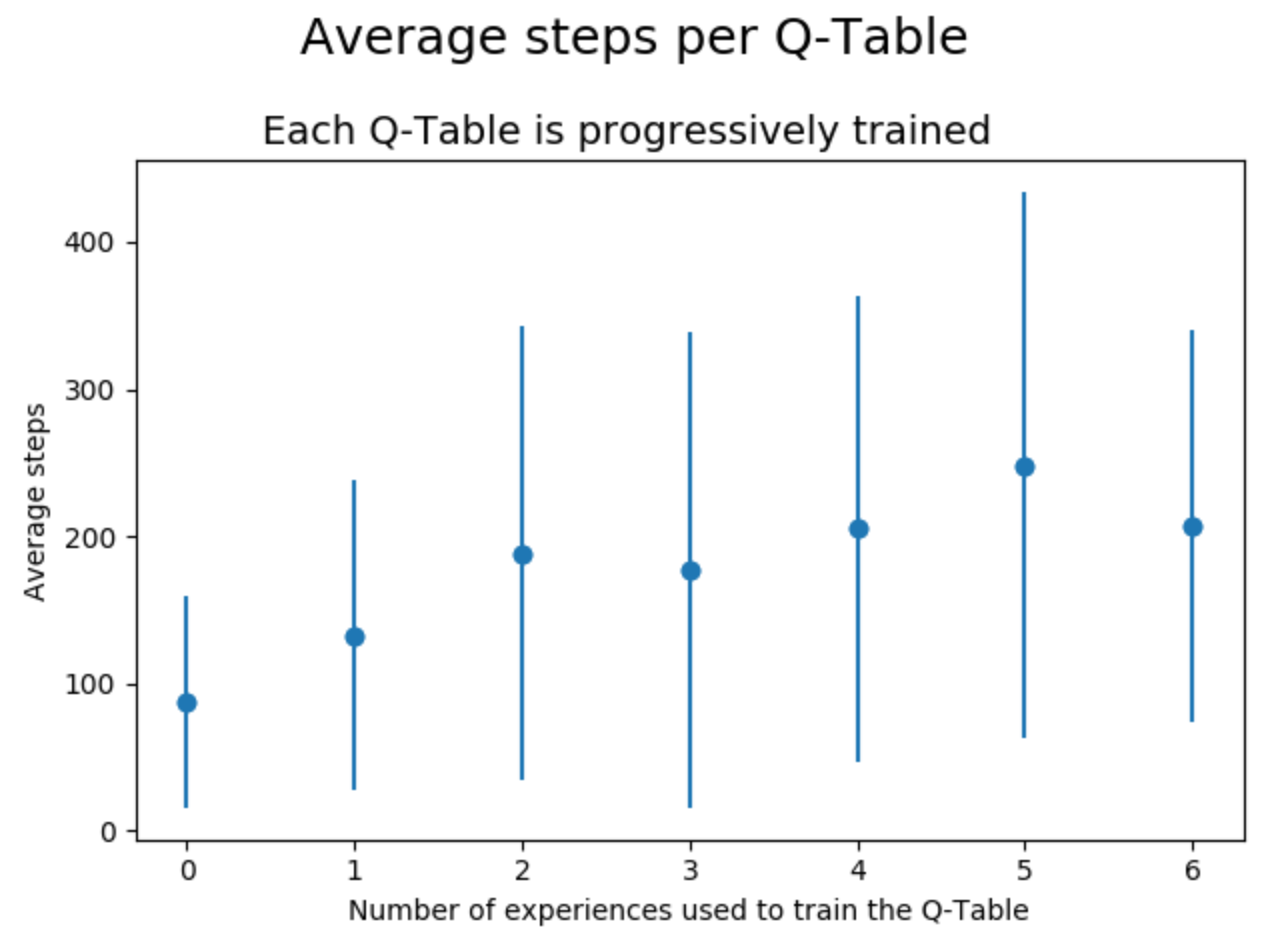
\includegraphics[scale=0.4]{Images/Average_steps/noise.png}
\caption{Average steps using Q-Table trained with a noisy signal.}
\label{fig:avg_steps_noise}
\end{figure}

Electroencephalographic signals have high inter-subject variability~\cite{Chavarriaga2014}.   This is evidenced in Figure~\ref{fig:transferlearning} where the agent training is performed by using rewards obtained by classifying epochs from one subject, but using a classifier which was trained using the brainwaves from a different subject.   No performance gain is evidenced, the agents learn nothing which implies that the reward information is useless.


\begin{figure}[h!]
\begin{subfigure}{0.5\textwidth}
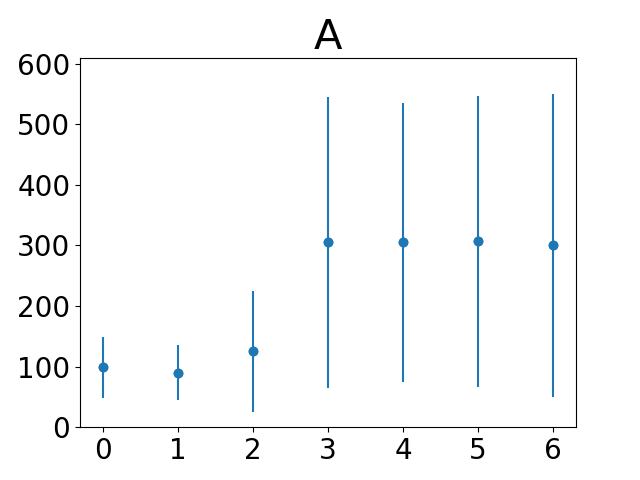
\includegraphics[scale=0.27]{Images/Average_steps/Ax.png}
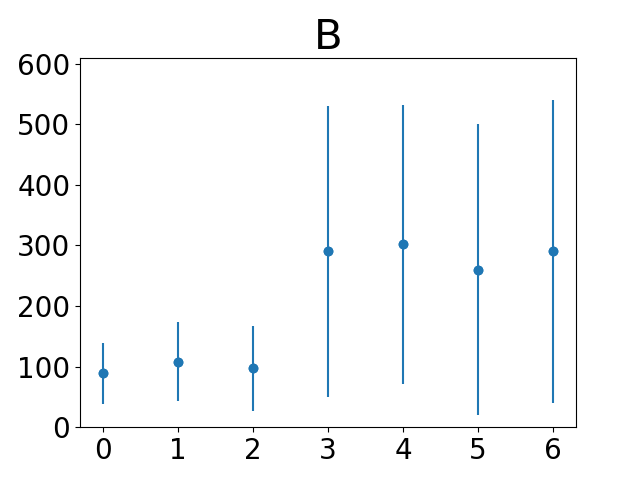
\includegraphics[scale=0.27]{Images/Average_steps/Bx.png}
\end{subfigure}
\caption{(A) Average steps using Q-table trained with experiences from subject 8 classified with a classifier trained with data from subject 6.  (B) Average steps using Q-table trained with experiences from subject 1 classified with a classifier trained with data from subject 3.}
\label{fig:transferlearning}
\end{figure}

Finally, Figure~\ref{fig:avg_steps_all} shows the result of training an agent with cumulative experiences from subjects 1,2,3,4,7, and 8.  It can be seen that the overall performance of the agent improves as long as there are more experiences to be used to train it, regardless if they were generated from the brainwaves classification from different subjects.  


\begin{figure}[h!]
\centering
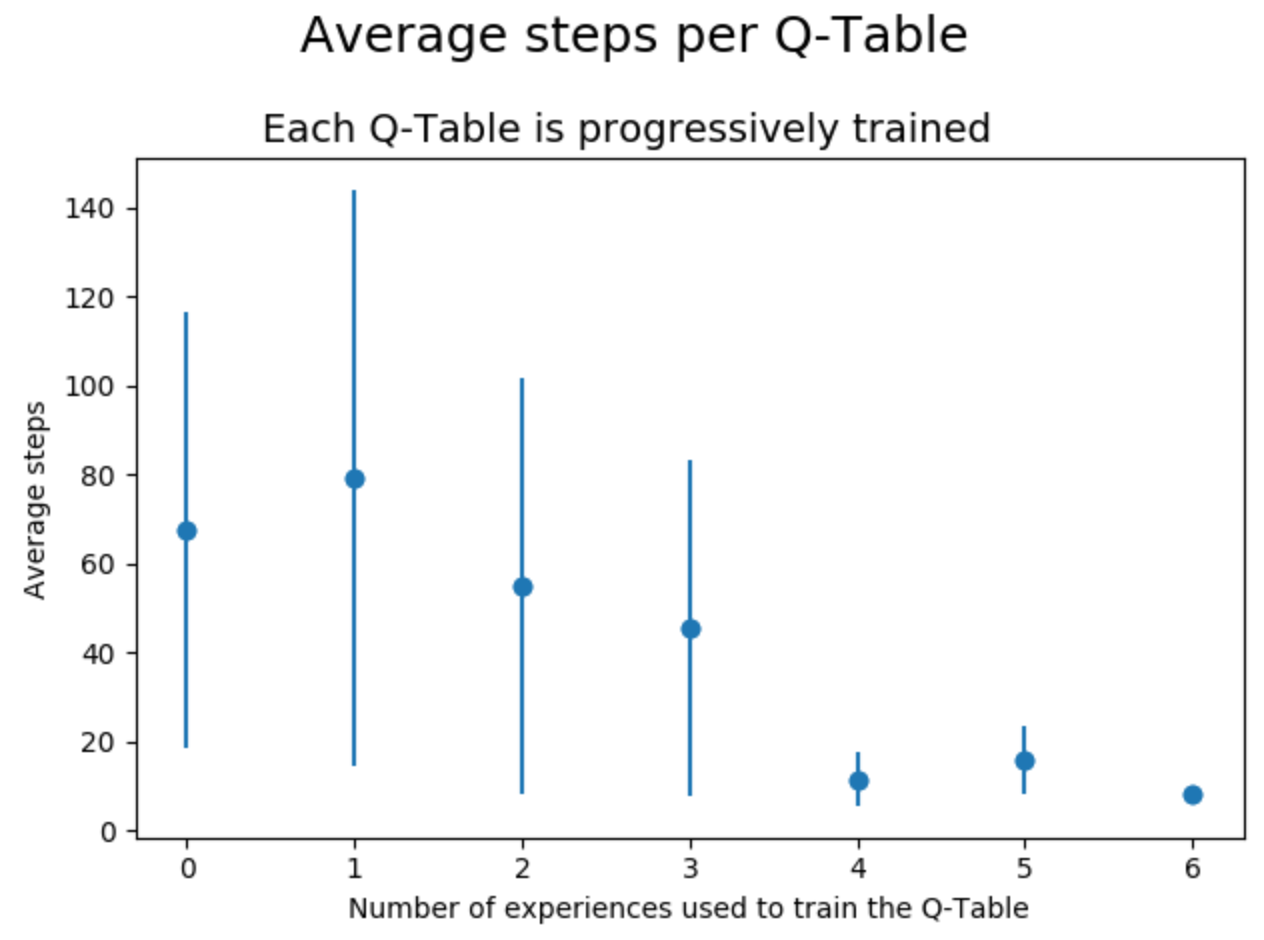
\includegraphics[scale=0.4]{Images/Average_steps/all.png}
\caption{Average steps using Q-Table trained with 6 experiences from different subjects.}
\label{fig:avg_steps_all}
\end{figure}

\section{Conclusion}
\label{conclusions}

%Enfatizar la idea de que la mejor métrica de la propia detección está dada por la propia capacidad del agente de minimizar su tarea, que hay un flujo de información que involucra la propia percepción de la persona.

This work aims to state whether ErrP signals could be used to train a gaming agent using reinforcement learning. The collected data show that ErrP signals can in fact be classified and used to train an agent effectively. 

This proposal tries to keep the system as simple as possible, emphasizing information flow from the subjective error perception of the human critic, through the reward generation using the signal processing and classification pipeline, and finally the Q-Table updating  to enhance the performance of the gaming agent.

%Enfatizar la idea de que la mejor métrica de la propia detección está dada por la propia capacidad del agente de minimizar su tarea, que hay un flujo de información que involucra la propia percepción de la persona.

%While classifying, the better performing classifier is Logistic Regression. One important aspect of the classification results is the low percentage of false positives (Figure~\ref{fig:confusionmatrix}), showing a high specificity.  It is not common that the agent learns that an action is wrong when in fact it is an action that takes it closer to the goal. On the other hand, the percentage of false negatives is generally higher, but this is not a serious issue since missing out on learning that an action is wrong does not lower the performance of the agent, but only means it will take more experiences to learn a correct path.

While classifying, the better performing classifier is Logistic Regression. One important aspect of the classification results is the low percentage of false positives (Figure~\ref{fig:confusionmatrix}), showing a high specificity.  It is not common that the agent learns that an action is wrong when in fact it is an action that takes it closer to the goal. On the other hand, the percentage of false negatives is generally higher.  However, even though this implies that the agent misses frequently that an action taken is wrong, this is not hindering the overall performance and the agent is still learning.

%However, even though this imply that the agent misses frequently that an action taken is wrong, this do not seems to be a serious issue because the agent improves its performance.


\begin{figure}[h!]
\begin{subfigure}{0.5\textwidth}
\centering
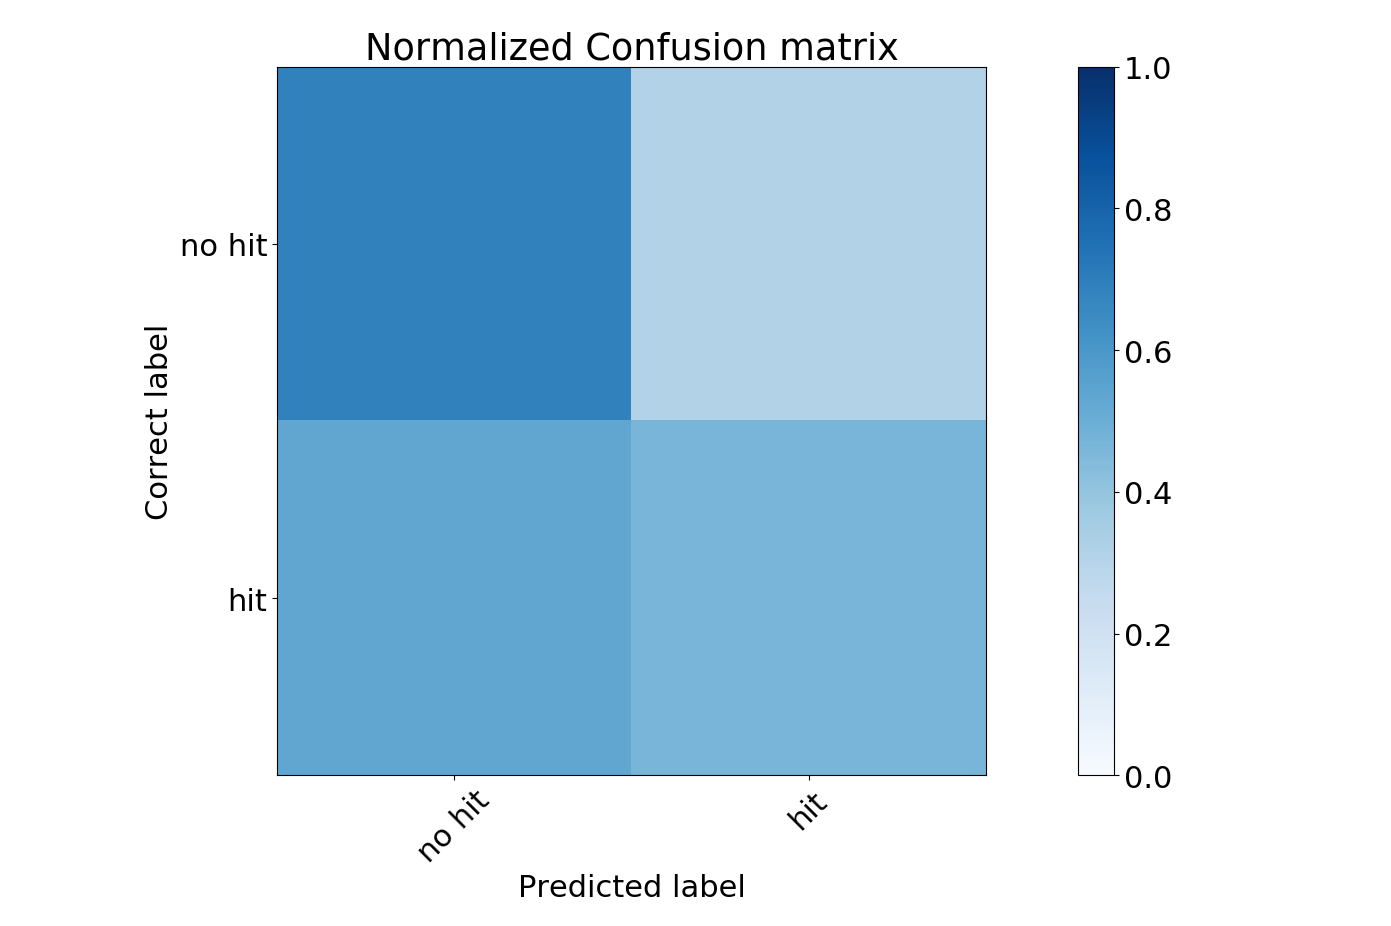
\includegraphics[scale=0.12]{Images/Classification_test/matrix_a.png}
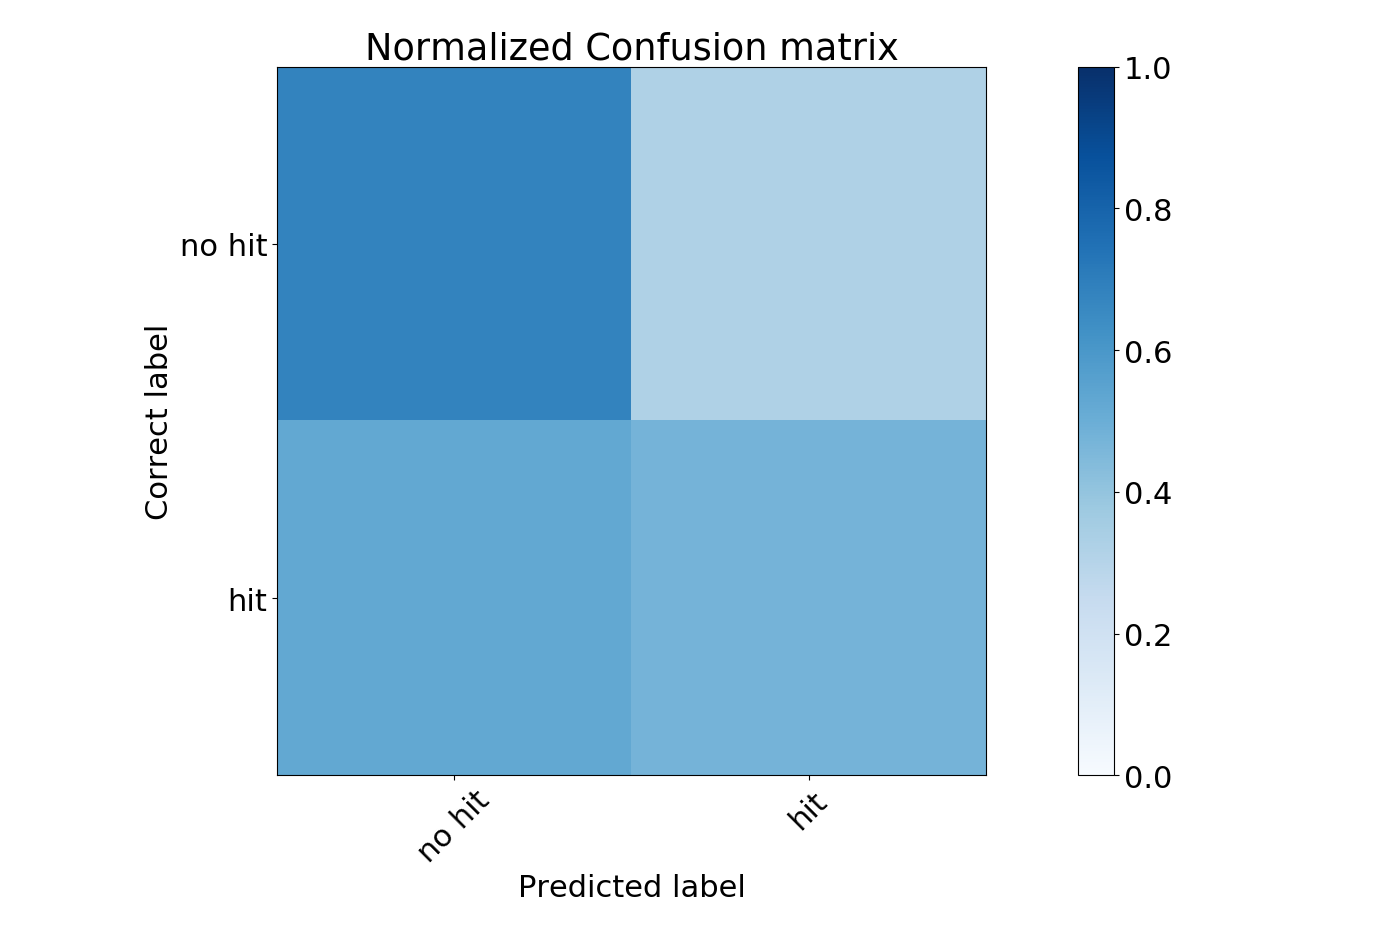
\includegraphics[scale=0.12]{Images/Classification_test/matrix_c.png}\\
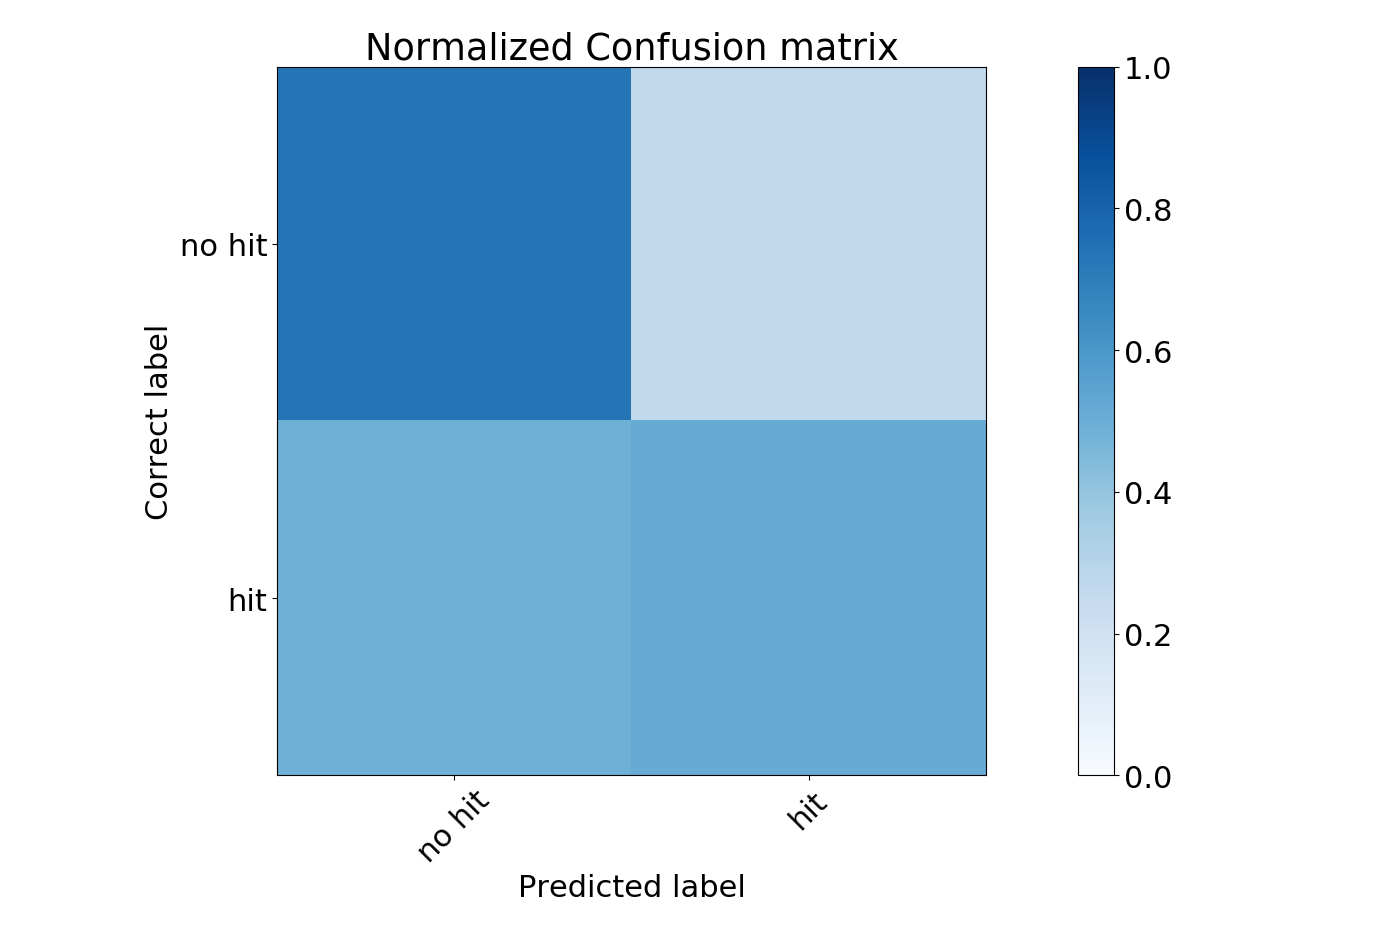
\includegraphics[scale=0.12]{Images/Classification_test/matrix_d.png}
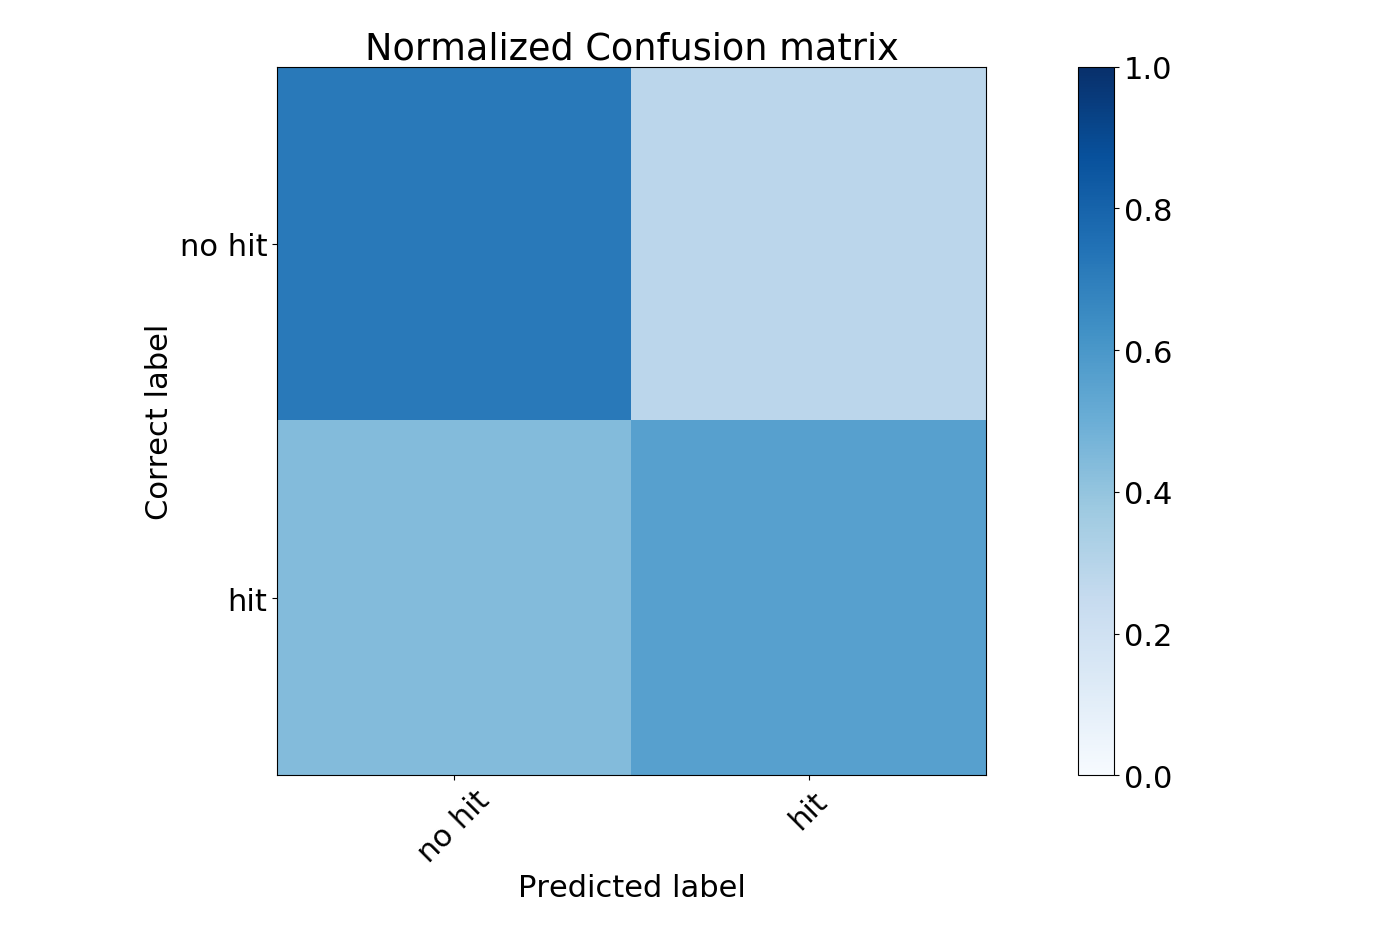
\includegraphics[scale=0.12]{Images/Classification_test/matrix_h.png}
\end{subfigure}
\caption{Confusion Matrix for subjects 1,3,4 and 8. Darker colors show higher values.  It can be seen the lower percentage of false positives (upper right corner of each chart).}
\label{fig:confusionmatrix}
\end{figure}

Once ErrP signals are identified they can be used to train an agent using a reinforcement learning algorithm. Brainwave sessions have a low amount of experiences in order to reduce fatigue from subjects. However data suggests that longer sessions are required in order to reach better classification scores, since more data is available in order to train the classifier. It can be seen that subjects with the largest amounts of data have the best classification. This can also be achieved designing a bigger game system that generates more samples with every session.

At the same time, effective agent training depends on the subject's data that was used to train it. Results show that training a classifier with data of one subject, but using it to classify the events of experiences of another subject does not lead to an improvement on the performance of the agent. Despite that, the rewards generated from different subjects can be used to train the same Q-Table to improve its performance, which may lead to strategies where the overall performance is improved based on the information from different human critics at the same time.

One additional aspect to remark is the robustness of the learning strategy based on Q-Learning~\cite{Bauer2015,Rubin2012}.  The obtained accuracy to discriminate ErrPs is low.  However, even with such a lower accuracy values, the RL algorithm was able to extract meaningful information from rewards that were helpful to improve the agent performance.  

Further work will be conducted in order to increase the complexity of the game to allow the possibility that the target position be dynamically changed.  In that case the agent would start to learn to follow the target, instead of learning to go to a specific static destination spot.  Additionally, the classifier could be enhanced to recognize more effectively the Error Potential~\cite{Iwane2017}.

Concluding, this research shows evidence that brain signals can be used as an interface between human and a gaming computer enabling an alternative communication with the system without explicit input from the user.



% if have a single appendix:
%\appendix[Proof of the Zonklar Equations]
% or
%\appendix  % for no appendix heading
% do not use \section anymore after \appendix, only \section*
% is possibly needed

% use appendices with more than one appendix
% then use \section to start each appendix
% you must declare a \section before using any
% \subsection or using \label (\appendices by itself
% starts a section numbered zero.)
%

% use section* for acknowledgment
\section*{Acknowledgment}

The authors would like to thank the Laboratory Centro de Inteligencia Computacional and to ITBA University.

\section*{Funding}
This work was supported by the grant ITBACyT-15 issued by ITBA University.

% Can use something like this to put references on a page
% by themselves when using endfloat and the captionsoff option.
\ifCLASSOPTIONcaptionsoff
  \newpage
\fi



% trigger a \newpage just before the given reference
% number - used to balance the columns on the last page
% adjust value as needed - may need to be readjusted if
% the document is modified later
%\IEEEtriggeratref{8}
% The "triggered" command can be changed if desired:
%\IEEEtriggercmd{\enlargethispage{-5in}}

% references section

% can use a bibliography generated by BibTeX as a .bbl file
% BibTeX documentation can be easily obtained at:
% http://mirror.ctan.org/biblio/bibtex/contrib/doc/
% The IEEEtran BibTeX style support page is at:
% http://www.michaelshell.org/tex/ieeetran/bibtex/
\bibliographystyle{IEEEtran}
\bibliography{References}
%
% <OR> manually copy in the resultant .bbl file
% set second argument of \begin to the number of references
% (used to reserve space for the reference number labels box)
% biography section
% 
% If you have an EPS/PDF photo (graphicx package needed) extra braces are
% needed around the contents of the optional argument to biography to prevent
% the LaTeX parser from getting confused when it sees the complicated
% \includegraphics command within an optional argument. (You could create
% your own custom macro containing the \includegraphics command to make things
% simpler here.)
%\begin{IEEEbiography}[{\includegraphics[width=1in,height=1.25in,clip,keepaspectratio]{mshell}}]{Michael Shell}
% or if you just want to reserve a space for a photo:

%\begin{IEEEbiography}{Michael Shell}
%Biography text here.
%\end{IEEEbiography}

% if you will not have a photo at all:
%\begin{IEEEbiographynophoto}{John Doe}
%Biography text here.
%\end{IEEEbiographynophoto}

% insert where needed to balance the two columns on the last page with
% biographies
%\newpage

%\begin{IEEEbiographynophoto}{Jane Doe}
%Biography text here.
%\end{IEEEbiographynophoto}

% You can push biographies down or up by placing
% a \vfill before or after them. The appropriate
% use of \vfill depends on what kind of text is
% on the last page and whether or not the columns
% are being equalized.

%\vfill

% Can be used to pull up biographies so that the bottom of the last one
% is flush with the other column.
%\enlargethispage{-5in}



% that's all folks
\end{document}


